%% ===========================================================================
%%  paper.en.tex  ·  MATCS: An Absolute Spatiotemporal Coordinate System for
%%                  Exact Quantification and Global Localization of Musical Events
%% ---------------------------------------------------------------------------
%%  Academic layout (musepaper-en.sty).  Style: English journal submission
%%  (consistent with Paper I).
%%
%%  English translation of the Chinese source paper.tex, which is left
%%  untouched.  Layout and terminology follow tools/glossary-en.md.
%%
%%  Source material:
%%    · 开发日志/开发日志.txt                      (theoretical derivation and narrative)
%%    · 开发日志/Muse_Agent：a profesional...md    (day 1 to day 8)
%%    · 开发日志/绝对Tick_变拍号补丁_v1.md         (general form under meter change)
%%    · 专利申请文件/最终稿件/说明书_终检版.txt     (MATCS formal technical scheme)
%%
%%  Compile: xelatex paper.en.tex, run at least twice for cross-references.
%% ===========================================================================
\documentclass[11pt,a4paper]{article}

\usepackage{musepaper-en}
\graphicspath{{figures/}}

%% ---------------------------------------------------------------------------
%%  Auxiliary environments used by this paper that musepaper-en.sty does not
%%  provide.  In the Chinese original they came from musepaper.sty
%%  (\begin{引述} and \begin{museCode}); the definitions below are local to this
%%  file, so musepaper-en.sty itself stays untouched.
%% ---------------------------------------------------------------------------
\usepackage{longtable}      % appendix glossary of terms
\usepackage{listings}       % \begin{museCode} code listings
\lstdefinestyle{musepaper}{%
  basicstyle = \ttfamily\small,
  keywordstyle = \color{museBlue}\bfseries,
  commentstyle = \color{black!45}\itshape,
  stringstyle = \color{teal!70!black},
  numbers = left, numberstyle = \tiny\color{black!35}, numbersep = 7pt,
  frame = single, framerule = 0.4pt, rulecolor = \color{black!25},
  breaklines = true, showstringspaces = false, tabsize = 2,
  columns = fullflexible, keepspaces = true,
  xleftmargin = 1.3em, framexleftmargin = 1.3em,
}
\lstnewenvironment{museCode}[1][]{\lstset{style=musepaper,#1}}{}

%% Quoted passage (the Chinese original's \begin{引述}): a plain indented block,
%% no rules and no background, in keeping with the no-boxes typography of
%% musepaper-en.sty.
\newenvironment{quotedpassage}{\begin{quote}\small}{\end{quote}}

%% Running head (English journal practice: a shortened title, centered)
\runninghead{MATCS: Absolute Spatiotemporal Coordinates of Musical Events}

\title{MATCS: An Absolute Spatiotemporal Coordinate System for\\
Exact Quantification and Global Localization of Musical Events}
\author{MOZUN}
\date{}

% ===========================================================================
%% ---------------------------------------------------------------------------
%%  Citation style (per the house rules of the Journal of the Central
%%  Conservatory of Music): all references appear as page-foot footnotes and no
%%  bibliography is appended.  The original \begin{thebibliography} has therefore
%%  been replaced by individual \footnote entries.
%%  ⚠️ The style requires the cited page number; wherever [to be verified]/[X] appears the
%%  translator must fill it in from the edition actually used.
%% ---------------------------------------------------------------------------
\begin{document}

% The title page carries neither running head nor page number (journal
% submission convention).
% Note: the titlepage environment is deliberately NOT used here --- it resets the
% page counter to 1 when the environment ends, while the title-page material
% (abstract and keywords) often spills onto page 2, so the spilled page and the
% table-of-contents page would print the same page number.  Natural flow is used
% instead.
\thispagestyle{empty}

% ---------------------------------------------------------------------------
% Title page
% ---------------------------------------------------------------------------
\begin{center}
{\sffamily\bfseries\fontsize{17}{21}\selectfont
 MATCS: An Absolute Spatiotemporal Coordinate System for\\[0.18em]
 Exact Quantification and Global Localization of Musical Events\par}

\vspace{0.9em}
{\normalsize MOZUN\par}
\vspace{0.35em}
{\small (Core Theory Project Group, Hefei 230000, Anhui, China)\par}
\vspace{0.25em}
{\small Correspondence: 368164331@qq.com\par}
\end{center}

\vspace{0.4em}
\begin{abstracten}

Music has long been regarded as ``the art of time'' --- transient, and hard to
measure exactly the way a painting can be. This paper argues that the difficulty
does not arise from the essence of music but from its metric: the notational
position expression ``bar $m$, beat $t$'' takes as its unit of measurement one
beat, which is itself parameterised by the time signature, so that the same
expression denotes different physical durations under different signatures.
\textbf{Change the time signature and the scale changes with it.}

It is necessary first to clarify what this paper does \textbf{not} claim. The
conversion between bar--beat--tick and absolute tick
($\mathrm{AbsTick}=\bigl((M-1)\cdot\mathrm{BPI}+(T-1)\bigr)\cdot\mathrm{TPB}$,
where $\mathrm{TPB}=\mathrm{PPQ}\times4/\mathrm{Denom}$) is already standard
practice in digital audio workstations, symbolic music libraries and game audio
engines (for example the \texttt{FBarMap} interface of the Unreal engine, and the
time conversions of MusPy and mido), and this paper \textbf{does not claim it as
new}.

The contribution of this paper is built on that conversion and consists of three
items. First, \textbf{a unified symbolic-level event criterion}: taking ``event
$=$ the instant at which the vertical value changes'' as the sole definition, so
that the detection of note onsets, legato, staccato and rests is reduced to one
and the same condition; rests are correspondingly redefined as \textbf{empty
events} (events whose pitch attribute is empty but whose onset and offset are
explicit), so that no undefined interval remains on the time axis. Second,
\textbf{the closed form under meter change and its degenerate property}: we give
a counterexample (the original formula errs by $3840$ ticks, exactly one $4/4$
bar), generalise the original formula to a piecewise summation form, and prove
that the original formula is the degenerate special case of that form when the
number of time-signature segments is $n=1$. Third, \textbf{a quantitative
characterisation of the applicability domain}: the parameter count of that form
grows linearly with the density of meter changes, and as that density approaches
``one change per bar'' the parameter count approaches the score itself and the
formula's leverage drops to zero, at which point the correct answer is not a
better formula but a paradigm shift (a time-signature event table $+$ binary
search).

On this basis, this paper gives the voice-separation mechanisms derived from
these coordinates (coarse register partition, recursive subdivision, the linking
method with its ``equidistance exclusion method'', and a \textbf{virtual bridge}
that bridges rest gaps), a quantitative form for event relations (legato,
staccato and large leaps unified as local quantities that can be counted pair by
pair), a precision analysis, and a single observation from a human--AI
collaboration.

\textbf{Scope.} This paper does not infer meter from the audio waveform --- that
assumption cannot be avoided; it does not give a strict upper bound on the
rounding error; it does not perform cross-implementation validation; and it does
not evaluate the musicality of the proposed generation architecture.
\end{abstracten}

\keywords{absolute tick; MATCS; spatiotemporal coordinate system;
variable time signature; event drawing; empty event; global localization}

\clearpage

\tableofcontents
\clearpage
\section{Introduction}
\subsection{Background and problem}

The processing of symbolic music --- editing, analysis, generation and retrieval ---
all takes ``the position of an event on the time axis'' as its common reference.
In a digital audio workstation (DAW), however, that reference is itself not stable:
the position expression used by musical notation, ``bar $m$, beat $t$'', is a
\textbf{relative} description whose unit of measurement, one beat, is defined by the
time signature. Once the time signature changes, the physical duration denoted by the
same expression changes with it --- \textbf{what changes is the ruler, not the thing
being measured}.

In engineering practice this property appears as three reproducible classes of
failure.

\textbf{(1) A time-signature switch causes positional drift.} The same material edits
normally under $4/4$, but after switching to $6/8$ its notes are systematically
displaced and must be corrected by hand one by one. The defect is ubiquitous in
existing DAWs, yet the industry has long accepted it as a ``normal phenomenon''.

\textbf{(2) Moving material invalidates the coordinates.} After material is moved
between tracks, the relative relations among its internal notes are unchanged, while
its project-level absolute positions all become invalid.

\textbf{(3) The landing point of generated output cannot be controlled.} When a melody
produced by a generative model is transferred into MIDI, its landing points are always
``close to but not equal to'' the target beat positions --- by ear one can judge that
the intention is bar $2$, beat $3$, but that intention cannot be reproduced exactly.

The third phenomenon is often attributed to insufficient model capability. That
attribution does not hold: generative models perform reliably on formal reasoning of
the kind $1+1=2$, and their failure here shows precisely that \textbf{the input
representation itself lacks computable precision}, not that their reasoning ability is
insufficient.

\subsection{Why this is a coordinate problem}

Push the analogy towards physical measurement: ``the third centimetre of the second
meter'' is well defined --- the ruler is fixed, and anyone measuring at any time
obtains the same result. Musical notation is not like that: ``bar $2$, beat $3$''
denotes a different tick length under $4/4$ and under $6/8$.

The substance of the problem is that the unit of measurement of that expression is
parameterised by the time signature. When the time signature changes within a piece,
the mapping ``bar number $\to$ tick'' is no longer linear but \textbf{piecewise
linear}. Existing implementations treat the tick as a \textbf{counting tool} within one
segment, whereas what is needed here is a \textbf{coordinate system} that spans
segments. The difference between the two is exactly what this paper addresses.

\begin{observation}
What musical notation lacks is not precision but an absolute ruler that is independent
of every variable.
\end{observation}

\subsection{Terminological clarification: irregular meter is not variable time signature}
\label{sec:terminology}

Before discussing this problem, a group of terms that have long been conflated must be
clarified. Existing accounts often call time signatures such as $5/8$ and $7/8$
``mixed meter'', and conclude on that basis that ``complex time signatures are already
covered''. That classification is misleading in tick mathematics.

\begin{table}[htbp]
\centering
\caption{The properties of four classes of time signature in tick mathematics}
\label{tab:meter}
\begin{tabular}{@{}p{2.4cm}p{3.2cm}p{2.2cm}p{6.4cm}@{}}
\toprule
\thd{Class} & \thd{Example} & \thd{BPI} & \thd{Does it introduce difficulty} \\
\midrule
Simple meter & $2/4$, $3/4$ & $2$, $3$ & No \\
Compound meter & $6/8$, $9/8$, $12/8$ & $6$, $9$, $12$ & No (each ``beat'' is a dotted note) \\
Irregular meter & $5/8$, $7/8$ & $5$, $7$ & \textbf{No} (unequal division within the bar) \\
\textbf{Variable time signature} & the signature changes mid-piece & \textbf{piecewise values} & \textbf{Yes} \\
\bottomrule
\end{tabular}
\end{table}

The point is this: for the first three classes in Table \ref{tab:meter} the BPI is a
\textbf{constant} throughout the whole piece, and however irregular its value may be
(whether $7/8 = 2+2+3$ or $5/8 = 3+2$), the bar length
$\mathrm{barLen}=\mathrm{BPI}\times\mathrm{TPB}$ never changes, so the coordinate
mapping is still linear. What is called ``irregular meter'' refers to an unequal
grouping \textbf{inside} the bar; the time signature itself does not change, and the
tick mathematics is entirely unaffected by the internal grouping.

\begin{observation}
What genuinely requires segmentation is \textbf{variable time signature}, that is, the
signature being changed mid-piece. And that is precisely the class that existing
validation never covered --- the original formula passes on $4/4$, $6/8$ and $7/4$ and
fails only under a changing signature (see section \ref{sec:counter}).
\end{observation}

\subsection{The contributions of this paper and what it does not claim}

It must first be made clear what this paper \textbf{does not claim}. The linear
conversion between bar--beat--tick and absolute tick is already standard practice in
digital audio workstations, symbolic music libraries and game audio engines: the Unreal
engine encapsulates it in the
\texttt{MusicTimestampBarBeatTickToTick} interface of its
\texttt{FBarMap} class, libraries such as MusPy and mido provide equivalent time
conversions, and the commit records of some open-source DAWs even contain entries that
specifically fix an ``off-by-one'' problem in that conversion. \textbf{This paper
therefore does not claim the conversion as a new mathematical result}; writing it as a
closed form merely provides an explicit base for the arguments that follow.

On that base, this paper makes three contributions.

\textbf{(1) A unified symbolic-level event criterion (section \ref{sec:event}).}
Taking ``event $=$ the instant at which the vertical value changes'' as the sole
definition reduces the detection of the four kinds of boundary --- note onset, legato,
staccato and rest --- to one and the same condition; rests are correspondingly
redefined as ``empty events'', and no undefined interval remains on the time axis. The
benefit of this item is testable --- four conditions that used to be handled separately
are replaced by a single criterion.

\textbf{(2) The closed form under a changing time signature and its degenerate
property (section \ref{sec:coord}).} We give a counterexample (the original formula
errs by $3840$ ticks, exactly one $4/4$ bar), generalise the single linear formula to a
piecewise summation form, and prove that the original formula is the degenerate special
case of that form when the number of time-signature segments is $n=1$. The practical
significance of the degenerate property is that replacing the implementation changes no
behavior of a single-signature project, so it can be deployed safely.

\textbf{(3) A quantitative characterisation of the applicability domain (section
\ref{sec:coord}).} The parameter count of that form grows linearly with the density of
time-signature changes; as the density approaches ``one change per bar'' the parameter
count approaches the score itself, and the formula's leverage relative to directly
listing the data drops to zero.
\textbf{Pointing out when a method should be abandoned is as important as giving the
method itself.}

On top of this, the paper gives several mechanisms derived from those coordinates ---
voice separation (section \ref{sec:voice}), the quantification of event relations
(section \ref{sec:relation}) and precision analysis (section \ref{sec:precision}).
They are \textbf{all derived quantities of the coordinate system rather than methods in
their own right}; this point is stated again at the beginning of each relevant chapter.

\subsection{What this paper does not cover}

To avoid misunderstanding, the following are outside the scope of this paper.

\begin{enumerate}[leftmargin=2.2em,itemsep=0.15em,topsep=0.2em]
  \item \textbf{It does not infer the beat or the time signature from the audio
        waveform.} That is a probabilistic estimation problem in Music Information
        Retrieval; this paper assumes that the segment table is supplied externally,
        and proposition \ref{prop:notick} shows that this assumption cannot be avoided.
  \item \textbf{It does not claim that musical aesthetics can be replaced by numbers.}
        This paper deals only with position and length, not with ``whether it sounds
        good''.
  \item \textbf{It does not give a strict upper bound on the rounding error under a
        changing time signature}; only experimental observation is offered
        (see section \ref{sec:limit}).
  \item \textbf{It does not provide cross-implementation validation.} The experiments
        were carried out on a single DAW only.
  \item \textbf{It does not validate the musicality of the proposed generation
        architecture.} The two worked examples in section \ref{sec:gen} verify the
        consistency of conservation and transformation, not the quality of the
        resulting piece.
\end{enumerate}

\subsection{Organisation of the paper}

Section \ref{sec:related} reviews related work and locates the difference between this
paper and existing work;
section \ref{sec:coord} establishes the core coordinate system;
sections \ref{sec:event}--\ref{sec:semantic} give corollaries at four levels;
section \ref{sec:collab} discusses the application of these corollaries in human--AI
collaboration;
section \ref{sec:exp} reports the implementation and the experiments;
section \ref{sec:disc} discusses limitations and boundaries.

\section{Related work}
\label{sec:related}
\subsection{Symbolic music representation}

There are two main lines of machine representation for symbolic music. The first is
MIDI and its standard file format
\footnote{MIDI Manufacturers Association, \emph{MIDI 1.0 Detailed Specification}, 1996, [to be verified: edition and cited page numbers]; E. Selfridge-Field (ed.), \emph{Beyond MIDI: The Handbook of Musical Codes}, Cambridge, MA: MIT Press, 1997, p. [X].}, which records performance information as a stream of event messages and whose time base is the product of ``pulses per quarter note'' (PPQ) and tempo, which does not correspond directly to the bar--beat structure of notation. The second is notation description languages such as MusicXML \footnote{M. Good et al., ``MusicXML: An Internet-Friendly Format for Sheet Music'', \emph{XML Conference and Exposition}, 2001, [to be verified: cited page numbers].} and Humdrum
\footnote{D. Huron, ``Humdrum and Kern: Selective Feature Encoding'', in \emph{Beyond MIDI: The Handbook of Musical Codes}, Cambridge, MA: MIT Press, 1997, pp. [X].}, which faithfully describe the visual and structural information of a score, but precisely for that reason their position expressions always remain tied to a time-signature context.

\begin{remark}
Each of the two representations has its strengths, but neither provides an absolute
position quantity that is independent of the time signature. What this paper deals with
is neither a performance message sequence nor a score document structure, but the
\textbf{mapping layer} between the two.
\end{remark}

\subsection{Computational models of beat, time signature and time}

The automatic inference of time signatures and beats is a classic problem in Music
Information Retrieval (MIR), covering subtasks such as beat tracking, downbeat
detection and meter detection, and the relevant methods are mostly based on statistical
estimation \footnote{M. Müller, \emph{Fundamentals of Music Processing}, Cham: Springer, 2015, p. [X].}. Such work differs from the present problem in one fundamental respect: MIR asks
``what might the time signature be'', which is a \textbf{statistical inference}
problem; this paper asks ``given the time signature, how is a position mapped exactly
to a coordinate'', which is a \textbf{deterministic computation} problem.

This yields a conclusion worth pointing out separately:

\begin{proposition}[Time-signature information cannot be recovered from ticks]
\label{prop:notick}
In raw MIDI or audio data, the time-signature map cannot be recovered uniquely from a
tick sequence.
\end{proposition}

\begin{proof}
The same tick data (for example $0,480,960,\dots,3360$) is interpreted as $1$ bar under
$4/4$, as $2$ bars under $2/4$, and as yet other structures under $3/4$ and $6/8$.
Multiple solutions exist, hence there is no unique solution, and the inverse problem is
ill-posed.
\end{proof}

Automatic inference of the time signature can therefore give only a statistical
estimate and no exact solution, which shows from the other side that the segment table
must be \textbf{externally supplied prior metadata} and cannot be recovered from the
coordinates (see section \ref{sec:domain} for details).

\subsection{Computational musicology toolchains}

The field of computational musicology has developed mature toolchains \footnote{M. S. Cuthbert and C. Ariza, ``music21: A Toolkit for Computer-Aided Musicology and Symbolic Music Data'', \emph{Proceedings of ISMIR 2010}, 2010, pp. [X].}; the formal description of tonal structure is represented by
generative grammar theory \footnote{F. Lerdahl and R. Jackendoff, \emph{A Generative Theory of Tonal Music}, Cambridge, MA: MIT Press, 1983, p. [X].}; and the mechanisms of temporal expectation for musical events have likewise been studied
systematically in psychology \footnote{D. Huron, \emph{Sweet Anticipation: Music and the Psychology of Expectation}, Cambridge, MA: MIT Press, 2006, p. [X].}. Most of this work discusses musical structure within an established
metrical context, whereas this paper treats the metrical context itself as the variable
to be dissolved.

\subsection{Absolute read-outs in DAW software}

Modern DAWs generally provide an absolute read-out of the form ``bar.beat.tick''
(for example REAPER's Big Clock window \footnote{Cockos Incorporated, \emph{REAPER User Guide and ReaScript API Reference}, [to be verified: edition, year and URL].}). That read-out is stable and unique within a project and does not drift with tempo
or with other time-signature segments; but when the time signature is changed
mid-project, if event coordinates are generated by a single linear formula such as
equation \eqref{eq:abs}, a systematic offset appears. The internal implementation of
DAW software uses a time-signature event table plus interval lookup, and does not
expose a closed-form expression for the case of a changing time signature
\footnote{See the preceding note.}. One part of this paper's work is to supply that
closed form, and at the same time to delimit its applicability boundary.

\subsection{Comparison with the standard MIDI tick}

The absolute time unit defined in this paper is not the same concept as the tick of the
MIDI standard; the differences between the two are given in Table \ref{tab:vsmidi}.

\begin{table}[htbp]
\centering
\caption{Comparison of the standard MIDI tick with the absolute time unit of this paper}
\label{tab:vsmidi}
\begin{tabular}{@{}p{3.5cm}p{5.2cm}p{5.2cm}@{}}
\toprule
\thd{Dimension} & \thd{Standard MIDI tick} & \thd{The absolute time unit of this paper} \\
\midrule
Relation to tempo & Coupled (a change in BPM directly affects the physical duration) & Decoupled (only the logical density changes) \\
Relation to the time signature & Implicitly dependent; must be inferred together with tempo and time signature & Explicitly decoupled; computed directly through TPB adaptation \\
Cross-segment consistency & Inconsistent; segments with different PPQ are not interchangeable & Consistent; forms a unified coordinate system within one project \\
Mathematical mapping & No direct mapping from ``bar.beat'' is given & Gives a ``minus-one shift $+$ time-signature adaptation'' mapping \\
Systematic architecture & None & Covers single-point localization, global recursion and structural verification \\
\bottomrule
\end{tabular}
\end{table}

\subsection{Limitations of DAW software itself}

Worth pointing out separately: the developers of DAW software are clearly aware of the
tick inconsistency problem. In documenting its absolute tick input facility, REAPER's
official documentation notes that because the software allows MIDI segments with
different PPQ to coexist, \textbf{a tick in one segment may not be equivalent to a tick
in another} \footnote{See the preceding note.}.

This remark delimits exactly the boundary of existing implementations: what they
provide is a counting tool \textbf{within a segment}, not a coordinate system
\textbf{unified across segments}. It is the latter that this paper supplies.

\subsection{Division of labour with Music Information Retrieval}

Beat tracking and onset detection in Music Information Retrieval take the audio
waveform as their object and output probability estimates; this paper takes a symbolic
event representation (such as MIDI) as its object and outputs deterministic
coordinates. The two do not compete: the former answers ``what might the time signature
be'', the latter answers ``given the time signature, how is a position mapped
exactly''. By proposition 1, the former cannot in principle give an exact solution,
which shows from the other side that the segment table must be supplied externally.

\subsection{Existing bar--beat--tick conversions}

This section sets out in one place the part that this paper \textbf{does not claim}, so
that readers do not misjudge the scope of its contribution. The linear conversion from
notational position to absolute tick is already a mature practice in several
engineering fields; Table \ref{tab:priorart} lists some of the implementations for
which public documentation exists.

\begin{table}[htbp]
\centering
\caption{Existing bar--beat--tick conversion implementations (not claimed as new by this paper)}
\label{tab:priorart}
\begin{tabular}{@{}p{3.4cm}p{2.4cm}p{7.6cm}@{}}
\toprule
\thd{Implementation} & \thd{Form} & \thd{Notes} \\
\midrule
Unreal Engine & the \texttt{FBarMap} class & Provides the \texttt{MusicTimestampBarBeatTickToTick} interface: bars and beats are both counted from 1 and ticks from 0, returning a 0-based absolute tick from the start of the piece; the documentation states this convention explicitly \\
MusPy & symbolic music library & implements the same mapping through a conversion between \texttt{resolution} (that is, PPQ) and metrical time \\
mido & MIDI library & \texttt{midifiles/units.py} provides conversion utilities between ticks and time units \\
madmom & MIR library & its MIDI IO contains an equivalent conversion between ticks and beat positions \\
the tempo map of an open-source DAW & source commit & commits exist that specifically fix the ``off-by-one'' problem between bar offset and beat arithmetic \\
\bottomrule
\end{tabular}
\end{table}

Two points are visible from Table \ref{tab:priorart}. First, the \textbf{content} of
that conversion is public prior art. Second, even the convention ``bars and beats
counted from 1, ticks counted from 0'' is not this paper's invention --- Unreal's
interface documentation states it explicitly. This paper therefore claims neither the
mathematical content of the conversion nor its counting convention.

What must be distinguished is an \textbf{implementation} from a \textbf{closed form}.
Most of the implementations above work by means of a \textbf{time signature map plus
interval lookup} (Unreal's documentation states that it is based on a time signature
map), and do not expose a closed-form expression for the case of a changing time
signature. The work of this paper here is \textbf{making explicit} rather than
discovery; its value lies not in the formula itself but in the criterion, the
degenerate property and the applicability boundary derived from it
(section \ref{sec:coord}).

\subsection{How this paper differs from existing work}

In summary, this paper does not claim that the quantifiability of music is a new
problem; it claims three things. First, the unit ``one beat'' must be relativised under
a changing time signature, and that relativisation has not been written out explicitly
in existing accounts. Second, the piecewise summation form that follows from it has a
definite degenerate property and can serve as a consistent extension of the original
formula. Third, the effective range of that form is constrained by the density of
time-signature changes, beyond which a paradigm shift is required.
Section \ref{sec:domain} gives a quantitative characterisation of that boundary.

% ---------------------------------------------------------------------------
%  Core chapter: the paper has exactly one core; every chapter below is a corollary of it
% ---------------------------------------------------------------------------
\section{The absolute time coordinate system: a position representation independent of the time signature}
\label{sec:coord}

This section is the technical foundation of the whole paper. Every conclusion in the
sections that follow can be derived directly from the three definitions given here
(the TPB conversion base, the absolute tick, and the bidirectional mapping), without
introducing any new independent assumption. This section therefore also carries the
responsibility of delimiting boundaries: wherever this coordinate system does not hold,
the corollaries built on it fail with it, so the applicability domain and the failure
mechanism are discussed here as well.

It is worth restating the conclusion of section \ref{sec:related}: the conversion in
this section is \textbf{not a new mathematical result} (see Table \ref{tab:priorart}).
The substantive work of this section is twofold --- generalising that conversion to a
piecewise summation form under a changing time signature and proving that the original
formula is its degenerate special case, and giving the quantitative boundary of its
applicability domain. Readers interested only in the contributions may go straight to
sections \ref{sec:counter} and \ref{sec:domain}.
\subsection{Observation: the stability of the scale}

In DAW software, a read-out of the form ``bar.beat.tick'' remains stable when the time
signature, the tempo or the position of the material changes. Table \ref{tab:clock}
gives the carry rules under three time signatures.

\begin{table}[htbp]
\centering
\caption{Counting carry rules under different time signatures}
\label{tab:clock}
\begin{tabular}{@{}lll@{}}
\toprule
\thd{Time signature} & \thd{Carry sequence} & \thd{Carry rule} \\
\midrule
$4/4$ & 1.1.00 $\to$ 1.2.00 $\to$ 1.3.00 $\to$ 1.4.00 $\to$ 2.1.00 & every four beats carry one bar \\
$6/8$ & 1.1.00 $\to$ 1.2.00 $\to \cdots \to$ 1.6.00 $\to$ 2.1.00 & every six beats carry one bar \\
$3/4$ & 1.1.00 $\to$ 1.2.00 $\to$ 1.3.00 $\to$ 2.1.00 & every three beats carry one bar \\
\bottomrule
\end{tabular}
\end{table}

This rule is isomorphic to a positional numeral system: the bar is the high-order
digit, the beat the low-order digit, and the numerator of the time signature determines
the carry radix. This observation suggests that the position expression can be
formalised as a purely counting mapping.

\subsection{The conversion base: from PPQ to TPB}

\begin{definition}[Number of numerical coordinate units per beat]
Let $\mathrm{PPQ}$ be the system's preset time resolution (pulses per quarter note) and
$\mathrm{Denom}$ the denominator of the current time signature; then the number of
numerical coordinate units per beat is defined as
\begin{equation}
  \label{eq:tpb}
  \mathrm{TPB} = \frac{\mathrm{PPQ}\times 4}{\mathrm{Denom}} .
\end{equation}
\end{definition}

Equation \eqref{eq:tpb} is the \textbf{unit calibration} of every coordinate
conversion in this paper: it translates the musicological unit ``one beat'' into a
number of machine-comparable numerical units. Table \ref{tab:tpb} gives the common
values ($\mathrm{PPQ}=960$).

\begin{table}[htbp]
\centering
\caption{Values of TPB ($\mathrm{PPQ}=960$)}
\label{tab:tpb}
\begin{tabular}{@{}lcccc@{}}
\toprule
\thd{Time signature} & \thd{Denom} & \thd{BPI} & \thd{TPB} & \thd{Bar length} \\
\midrule
$4/4$ & 4 & 4 & 960 & 3840 \\
$3/4$ & 4 & 3 & 960 & 2880 \\
$6/8$ & 8 & 6 & 480 & 2880 \\
\bottomrule
\end{tabular}
\end{table}

\begin{remark}
$\mathrm{TPB}$ corresponds one-to-one with the time signature: different signatures
correspond to different values, and the same signature corresponds to the same value in
any project. It must be stressed that this correspondence presupposes \textbf{adopting
the DAW's convention for ``one beat''} --- under $6/8$ the DAW defines one beat as an
eighth note ($\mathrm{TPB}=480$), whereas in music theory $6/8$ is usually read as two
dotted quarter notes. Adopt a different convention for the beat unit and the read-out
changes with it (see precondition C in section \ref{sec:domain}).
\end{remark}
\subsection{The definition of the absolute tick}

\begin{definition}[Absolute tick]
\label{def:defn}
Let the start of the project be $1.1.00$, let $M$ denote the bar number, $T$ the beat
number and $\mathrm{BPI}$ the number of beats per bar; then the absolute tick of the
position $(M,T)$ is defined as
\begin{equation}
  \label{eq:abs}
  \mathrm{AbsTick}(M,T) = \bigl((M-1)\cdot \mathrm{BPI} + (T-1)\bigr)\times \mathrm{TPB}.
\end{equation}
\end{definition}

The reasoning behind equation \eqref{eq:abs} is: $(M-1)\cdot\mathrm{BPI}$ is the total
number of beats before the current bar, $(T-1)$ is the number of beats already elapsed
within the current bar, and multiplying by $\mathrm{TPB}$ converts the result into a
number of absolute ticks.

The two $-\,1$ terms in definition \ref{def:defn} are not a mathematical convention but
the alignment of the counting origins: a notational position is counted from $1$, while
the tick count starts from $0$. Omitting that alignment introduces a systematic bias of
``one bar plus one beat'', as Table \ref{tab:minusone} shows.

\begin{table}[htbp]
\centering
\caption{The effect of aligning the counting origins ($4/4$, $\mathrm{BPI}=4$, $\mathrm{TPB}=960$)}
\label{tab:minusone}
\begin{tabular}{@{}lccc@{}}
\toprule
\thd{Position} & \thd{Unaligned} & \thd{Aligned} & \\
\midrule
\texttt{1.1.00} & $(1\times 4+1)\times 960=4800$ & $((1-1)\times 4+(1-1))\times 960=0$ & \checkmark \\
\texttt{2.1.00} & $(2\times 4+1)\times 960=8640$ & $((2-1)\times 4+(1-1))\times 960=3840$ & \checkmark \\
\texttt{1.3.00} & $(1\times 4+3)\times 960=6720$ & $((1-1)\times 4+(3-1))\times 960=1920$ & \checkmark \\
\bottomrule
\end{tabular}
\end{table}

\begin{remark}[The status of the ``minus one'']
The $-\,1$ in equation \eqref{eq:abs} is a \textbf{translation rule} rather than a
mathematical rule: it maps a human coordinate counted from $1$ onto a machine
coordinate counted from $0$. Remove that shift and every position moves by ``one bar
plus one beat'' as a whole.
\end{remark}

\subsection{Event coordinatization}

Taking the absolute tick as the horizontal axis of a Cartesian coordinate system and
the event pitch $P$ as the vertical axis gives the two-dimensional event coordinate:
\begin{equation}
  \label{eq:event}
  \mathrm{Event} = (\mathrm{AbsTick},\; P).
\end{equation}

Every event therefore has a unique start and end absolute coordinate
$(\mathrm{Start}_{\mathrm{absTick}},\;\mathrm{End}_{\mathrm{absTick}},\;P)$, whose
localization does not depend on the time-signature context. Equation \eqref{eq:event}
provides a unified mathematical framework for voice separation, melody tracking and
harmonic analysis.

\subsection{Bidirectional mapping}

The inverse mapping can be derived from equation \eqref{eq:abs}. Writing
$\mathrm{TotalBeats}=\mathrm{AbsTick}/\mathrm{TPB}$, we have
\begin{align}
  \mathrm{TotalBeats} &= \mathrm{AbsTick} / \mathrm{TPB}, \label{eq:tb}\\
  M &= \bigl\lfloor \mathrm{TotalBeats} / \mathrm{BPI} \bigr\rfloor + 1, \label{eq:invM}\\
  T &= \bigl(\mathrm{TotalBeats} \bmod \mathrm{BPI}\bigr) + 1 . \label{eq:invT}
\end{align}

Equation \eqref{eq:abs} together with equations \eqref{eq:tb}--\eqref{eq:invT} forms a
complete inference loop, ensuring that the localization process is unambiguous and
traceable.

\subsection{Verification}

Under $6/8$ ($\mathrm{BPI}=6$, $\mathrm{Denom}=8$, $\mathrm{PPQ}=960$, hence
$\mathrm{TPB}=480$) take \texttt{4.1.00} for the forward computation:
\[
\bigl((4-1)\times 6+(1-1)\bigr)\times 480 = 18\times 480 = 8640 .
\]
Substituting back into equations \eqref{eq:invM}--\eqref{eq:invT} gives a total of
$8640/480=18$ beats, $M=\lfloor 18/6\rfloor+1=4$ and $T=(18 \bmod 6)+1=1$, that is
\texttt{4.1.00}, which agrees with the input. Table \ref{tab:verify} summarises the
verification data.

\begin{table}[htbp]
\centering
\caption{Bidirectional verification ($4/4$ and $6/8$)}
\label{tab:verify}
\begin{tabular}{@{}llccccc@{}}
\toprule
\thd{Time signature} & \thd{Input position} & \thd{$M$} & \thd{$T$} & \thd{Absolute tick} & \thd{Inferred result} & \thd{Consistent} \\
\midrule
$4/4$ & \texttt{2.3.00} & 2 & 3 & 5760  & \texttt{2.3.00} & \checkmark \\
$6/8$ & \texttt{4.1.00} & 4 & 1 & 8640  & \texttt{4.1.00} & \checkmark \\
$6/8$ & \texttt{5.3.00} & 5 & 3 & 12480 & \texttt{5.3.00} & \checkmark \\
\bottomrule
\end{tabular}
\end{table}

\subsection{A changing time signature: counterexample and generalisation}
\label{sec:counter}
\subsubsection{The implicit assumption of the original formula}

Consider the $(M-1)\cdot\mathrm{BPI}$ term in equation \eqref{eq:abs}: it uses the
\textbf{current $\mathrm{BPI}$ to multiply the total number of bars}. This step assumes
that all bars in the project have exactly the same length.

As long as that assumption holds, equation \eqref{eq:abs} is \textbf{exact} (not an
approximation), and the verifications above on $4/4$, $6/8$ and $7/4$ are all valid.
But as soon as the time signature changes mid-project, the assumption is broken.

\subsubsection{Counterexample}

\begin{figure}[htbp]
\centering
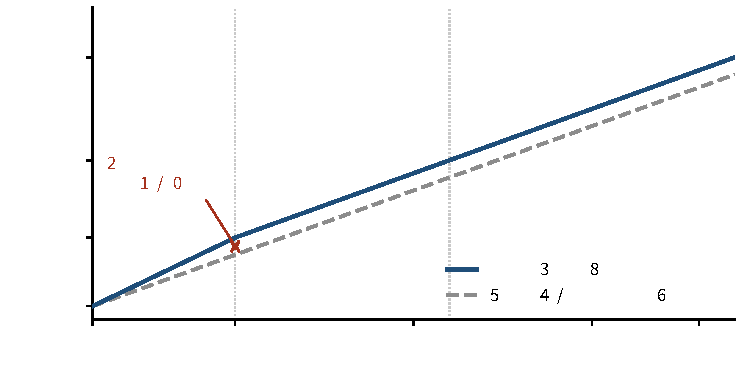
\includegraphics[width=0.78\textwidth]{fig-pwl.pdf}
\caption{The deviation between the single linear formula and piecewise summation under
a changing time signature. The dashed line is the original formula (multiplying by the
BPI of segment 2), the solid line is the true piecewise accumulation; the two separate
from bar $5$ onwards, and the deviation is constantly $3840$ ticks, exactly one $4/4$
bar.}
\label{fig:pwl}
\end{figure}

Consider a project with three time-signature segments, with the parameters given in
Table \ref{tab:segdata}.

\begin{table}[htbp]
\centering
\caption{Settings of the meter-changing project ($\mathrm{PPQ}=960$)}
\label{tab:segdata}
\begin{tabular}{@{}llcccc@{}}
\toprule
\thd{Segment} & \thd{Bar range} & \thd{Time signature} & \thd{TPB} & \thd{Bar length} \\
\midrule
Segment 1 & $1$--$4$   & $4/4$ & 960 & $4\times 960=3840$ \\
Segment 2 & $5$--$10$  & $3/4$ & 960 & $3\times 960=2880$ \\
Segment 3 & $11$--$18$ & $6/8$ & 480 & $6\times 480=2880$ \\
\bottomrule
\end{tabular}
\end{table}

We want the absolute tick of bar $5$, beat $1$ (\texttt{5.1.00}). Substituting into
equation \eqref{eq:abs} and using the $\mathrm{BPI}=3$ of segment 2:
\[
\bigl((5-1)\times 3 + (1-1)\bigr)\times 960 = 4\times 3\times 960 = 11520 \quad(\text{wrong}).
\]
Whereas by piecewise accumulation, the first $4$ bars are $4/4$ and should give
\[
4\times 4\times 960 = 15360 \quad(\text{right}).
\]

\begin{observation}
The error is $15360-11520 = 3840$ ticks, \textbf{exactly one $4/4$ bar}.
The cause is that the first $4$ bars were in fact $4/4$ ($4$ beats per bar) but were
recomputed once by the original formula with the $\mathrm{BPI}=3$ of segment 2.
\end{observation}

The feature that the error is ``exactly equal to one bar'' deserves attention: it shows
that the deviation is not rounding noise but structural --- the original formula
mistakes a piecewise linear mapping for a straight line.

\subsubsection{Mathematical diagnosis}

Equation \eqref{eq:abs} treats ``bar number $\to$ tick'' as a linear mapping solvable by
a single multiplication:
\begin{equation}
  \mathrm{Tick}(M) = k\cdot M + c \qquad(\text{a straight line}).
\end{equation}
But once the time signature changes, that mapping is \textbf{piecewise linear} --- each
segment has a different slope, and the slope of the $k$-th segment is
\begin{equation}
  \label{eq:slope}
  \text{slope}_k = \mathrm{BPI}_k \times \mathrm{TPB}_k .
\end{equation}

\begin{observation}[A key metaphor]
The original formula takes the coordinate function to be a straight line, whereas it is
in fact a polyline. For a \textbf{straight line} one multiplication suffices
everywhere; for a \textbf{polyline} only \textbf{piecewise summation} works.
\end{observation}

\subsubsection{The general form of piecewise summation}

Suppose the project is divided into $m$ time-signature segments, with the parameters of
the $s$-th segment as given in Table \ref{tab:seg}.

\begin{table}[htbp]
\centering
\caption{Notation of the segment table}
\label{tab:seg}
\begin{tabular}{@{}ll@{}}
\toprule
\thd{Symbol} & \thd{Meaning} \\
\midrule
$n_k$    & the number of bars governed by segment $k$ \\
$p_k$    & beats per bar in segment $k$ ($=$ the numerator of the time signature) \\
$d_k$    & the denominator of the time signature of segment $k$ \\
$t_k$    & the number of ticks per beat in segment $k$ $=$ $\mathrm{PPQ}\times 4 / d_k$ \\
$\ell_k$ & the number of ticks per bar in segment $k$ $=$ $p_k \times t_k$ \\
\bottomrule
\end{tabular}
\end{table}

The segment start $S_s$ is a cumulative quantity:
\begin{equation}
  \label{eq:segstart}
  S_1 = 0,\qquad S_s = \sum_{k=1}^{s-1} n_k \,\ell_k .
\end{equation}
Writing $A_s=\sum_{k<s} n_k$ for the total number of bars in the preceding segments, the
combined general form is
\begin{equation}
  \label{eq:master}
  \mathrm{AbsTick}(M,T) = \sum_{k<s} n_k \,\ell_k
  + \bigl((M-A_s-1)\,p_s + (T-1)\bigr)\,t_s .
\end{equation}
\begin{figure}[htbp]
\centering
\begin{schematic}
\begin{verbatim}
tick:   0                15360              32640
        |                  |                  |
        +--- seg 1 ---+---- seg 2 ----+--- seg 3 --->
        |  4 bars     |  6 bars       |  8 bars
        |  3840/bar   |  2880/bar     |  2880/bar
       S1=0          S2=15360        S3=32640
\end{verbatim}
\end{schematic}
\caption{The structure of the time-signature segments. The slope changes at bars $5$
and $11$, so the cumulative quantity must be summed piecewise.}
\label{fig:segments}
\end{figure}

\begin{remark}[The demotion of the ``minus one'']
Compare equation \eqref{eq:abs} with equation \eqref{eq:master}: the bar term changes
from $(M-1)$ to $(M-A_s-1)$. \textbf{The ``minus one'' has not changed, but it has been
demoted from a ``global minus one'' to a ``within-segment minus one''.}
\end{remark}

\subsubsection{The degeneracy theorem}

\begin{theorem}[Degeneracy]
When the number of segments is $n=1$, the general form \eqref{eq:master} degenerates to
the original formula \eqref{eq:abs}.
\end{theorem}

\begin{proof}
With a single segment $A_1=0$ and $\sum_{k<1}(\cdot)=0$; substituting into
\eqref{eq:master} gives
$\mathrm{AbsTick}(M,T)=\bigl((M-1)\cdot\mathrm{BPI}+(T-1)\bigr)\cdot\mathrm{TPB}$,
which agrees with \eqref{eq:abs} term by term.
\end{proof}

This conclusion shows that equation \eqref{eq:master} is a \textbf{domain extension} of
the original formula rather than a replacement: the domain of the original formula is
$n=1$ segment, while the domain of the general form is any finite number of segments.
In a single-signature project, replacing the implementation changes no existing
behavior, so it can be deployed safely.

\begin{remark}[An assumption becomes a variable]
The original formula hard-codes the \textbf{assumption} ``one and the same time
signature throughout the piece'' into the formula; the general form turns that
assumption itself into a \textbf{variable} (the segment table). \textbf{Once the
assumption becomes a variable, the special case grows into the general form.}
\end{remark}

\subsubsection{Verification after generalisation}

For the project of Table \ref{tab:segdata}, we computed equation \eqref{eq:master}
point by point and compared the results with measurements from the DAW; the results are
given in Table \ref{tab:verify2}.

\begin{table}[htbp]
\centering
\caption{Measured comparison for the meter-changing project}
\label{tab:verify2}
\begin{tabular}{@{}lcccc@{}}
\toprule
\thd{Position} & \thd{Original formula} & \thd{General form} & \thd{Measured in the tool} & \thd{Verdict} \\
\midrule
\texttt{5.1.00}  & 11520 & \textbf{15360} & 15360 & the general form is correct \\
\texttt{9.2.00}  & ---    & \textbf{27840} & 27840 & the general form is correct \\
\texttt{11.1.00} & ---    & \textbf{32640} & 32640 & the general form is correct \\
\bottomrule
\end{tabular}
\end{table}

The hand calculation for \texttt{9.2.00} is as follows:
\begin{align*}
  S_2 &= 15360,\\
  \text{within segment} &= (M-A_2-1)\cdot p_2 + (T-1) = (9-4-1)\times 3 + (2-1) = 13,\\
  \Delta &= 13\times 960 = 12480,\\
  \text{total} &= 15360 + 12480 = 27840 \;\checkmark .
\end{align*}

\subsubsection{Rounding error}

Equation \eqref{eq:tpb} must be rounded when the denominator is not a power of $2$, and
the error may accumulate with the number of segments. When
$d_k\in\{2,4,8,16,32\}$ and $\mathrm{PPQ}=960$ the division is exact and there is no
error; for rare denominators rounding is required. It is advisable to choose
$\mathrm{PPQ}$ as a high power ($960 = 2^6\times 3\times 5$, divisible down to $/32$) in
order to reduce the probability of that error occurring. This section gives observation
only; a strict proof of the error bound is left to future work (see
section \ref{sec:limit}).

\subsection{Precision analysis}
\label{sec:precision}
The precision of the absolute coordinate is not determined by human perception but by
the numerical resolution of the system. At $\mathrm{PPQ}=960$, one beat corresponds to
$960$ ticks, that is $1\ \mathrm{tick} \approx 1/960$ beat. Converted into physical
time, this gives Table \ref{tab:prec}.

\begin{table}[htbp]
\centering
\caption{Temporal precision at different resolutions ($120$ BPM)}
\label{tab:prec}
\begin{tabular}{@{}lcc@{}}
\toprule
\thd{PPQ} & \thd{Time corresponding to 1 tick} & \thd{Relative to one beat at $120$ BPM} \\
\midrule
$960$   & $\approx 0.5208$ ms & $1/960$ \\
$9600$  & $\approx 0.052$ ms  & $1/9600$ \\
$96000$ & $\approx 0.0052$ ms & $1/96000$ \\
\bottomrule
\end{tabular}
\end{table}

\begin{observation}
At the highest setting this precision already exceeds the resolving limit of human
hearing, but its significance lies elsewhere: \textbf{this precision is determined not
by human perception but by the computational precision of the computer.} The coordinate
system itself has no capability ceiling, only parameter settings.
\end{observation}

For reference, this system precision can be compared with the temporal control ability
of human performance. The temporal control precision of a top performer is on the order
of $10\sim 20$ ms; at $120$ BPM one beat is $500$ ms, so that precision is about
$1/50$ beat. $\mathrm{PPQ}=960$ corresponds to $1/960$ beat $\approx 0.5$ ms, already
about $20$ times that magnitude; and $\mathrm{PPQ}=96000$ gives a precision of
$0.005$ ms, entirely beyond any human perceptual ability.

\begin{remark}
The point of the comparison above is not that ``machines are more accurate than
people'' but rather that, under this system, the source of error is \textbf{parameter
setting} rather than a \textbf{capability ceiling}. Whether higher precision ought to be
pursued is a question bound up with aesthetics and use. A note deviating from the
standard grid by $0.0.12$ can be read either as ``not accurate enough'' or as ``this is
simply how he phrases it'' --- this system is only responsible for measuring it out.
\end{remark}

Accordingly, several modifiers in traditional accounts that can be conveyed only by
feeling can acquire a quantitative counterpart:

\begin{table}[htbp]
\centering
\caption{From qualitative modifiers to quantitative offsets}
\label{tab:qualitative}
\begin{tabular}{@{}ll@{}}
\toprule
\thd{Traditional expression} & \thd{Coordinatized expression} \\
\midrule
``a little faster'' & $3$ ticks earlier \\
``a little looser'' & $2$ ticks longer \\
``not accurate enough'' & offset by $6$ ticks \\
\bottomrule
\end{tabular}
\end{table}

\begin{remark}
Table \ref{tab:qualitative} does not mean that aesthetic judgement can be replaced by
numbers; it shows only that once position and length are coordinatized,
\textbf{descriptions of them} can become precise. ``Precise'' and ``pleasant to hear''
are two different questions, and this system answers only the former.
\end{remark}

\subsection{Applicability domain and failure mechanism}
\label{sec:domain}
This section gives the applicability boundary of the form. Such self-limitation is not
common in technical reports, but it is necessary for engineering deployment --- a
computational interface that does not know when it fails is dangerous.

\subsubsection{Time-signature change density}

The validity of equation \eqref{eq:master} decays with the density of time-signature
changes. Table \ref{tab:domain} compares three classes of scenario.

\begin{table}[htbp]
\centering
\caption{The applicability domain partitioned by time-signature change density}
\label{tab:domain}
\begin{tabular}{@{}p{4.0cm}p{2.2cm}p{3.6cm}p{4.4cm}@{}}
\toprule
\thd{Scenario} & \thd{Original formula} & \thd{General form} & \thd{Correct solution} \\
\midrule
A single time signature & correct & correct (degenerate equivalence) & either one \\
A few meter changes & fails & correct & the general form \\
Ban-shi change / free meter (sanban) / dense meter change & fails & fails & a time-signature event table $+$ binary search \\
\bottomrule
\end{tabular}
\end{table}

\subsubsection{Parameter complexity}

\begin{figure}[htbp]
\centering
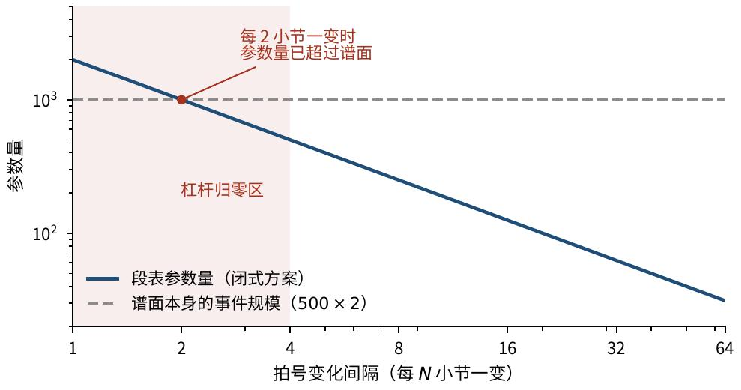
\includegraphics[width=0.78\textwidth]{fig-density.pdf}
\caption{The growth of the parameter count with time-signature change density (a project
of $500$ bars, on average $2$ events per bar). The horizontal axis is ``one change every
$N$ bars'', the vertical axis is logarithmic. The segment-table parameter count is
plotted as a continuous value --- the actual number of segments must be rounded, and
rounding would turn the curve into a staircase, omitted here so that the trend stays
visible. As the density rises the parameter count grows with it, and at one change
every $2$ bars it exceeds the event count of the score itself, whereupon the leverage of
the closed form relative to directly listing the data drops to zero.}
\label{fig:density}
\end{figure}

\begin{table}[htbp]
\centering
\caption{The growth of the parameter scale with time-signature change density}
\label{tab:params}
\begin{tabular}{@{}ll@{}}
\toprule
\thd{Scenario} & \thd{Parameter count} \\
\midrule
A single time signature & $\approx 3$ \\
$3$ meter-change segments & $3\times 4 = 12$ \\
dense meter change (one change every $2$ bars, $500$ bars) & $\approx 1000$ \\
\bottomrule
\end{tabular}
\end{table}

The parameter count grows \textbf{linearly} with the time-signature change density; its
curve is shown in Figure \ref{fig:density}, and Table \ref{tab:params} gives three
representative values.

\begin{observation}[Failure mechanism]
As the time-signature change density approaches ``one change per bar'', the parameter
scale approaches the score itself and the formula's leverage relative to directly
listing the data drops to zero.
\end{observation}

The correct answer here is not a ``better formula'' but a \textbf{paradigm shift}: store
a time-signature event table and change the query to an $O(\log n)$ binary search. This
is exactly how mainstream DAWs implement it, and none of them exposes a closed-form
formula for the case of a changing time signature \footnote{See the preceding note.}.

\begin{remark}[The position of this form]
Equation \eqref{eq:master} is an $O(1)$ computational interface for the ``low-density
meter change'' scenario. It is not a mathematical discovery, nor a general solution,
but a small tool with clearly defined boundaries; its upper bound of value is
determined by the time-signature change density.
\end{remark}

\subsubsection{The irreplaceability of the reverse mapping}

The value of equations \eqref{eq:abs} and \eqref{eq:master} is not symmetric between
the forward and the reverse direction:

\begin{table}[htbp]
\centering
\caption{Replaceability in the forward and reverse directions}
\label{tab:asym}
\begin{tabular}{@{}lll@{}}
\toprule
\thd{Direction} & \thd{Form} & \thd{Can it be replaced by hand} \\
\midrule
Forward & $\mathrm{Position} \to \mathrm{AbsTick}$ & yes, even by hand calculation \\
Reverse & $\mathrm{AbsTick} \to \mathrm{Position}$ & \textbf{no}, it must rely on the cumulative boundaries $S_s$ \\
\bottomrule
\end{tabular}
\end{table}

The reason is that the relation between position and tick is a piecewise linear,
strictly monotonic bijection, and the reverse solution lands precisely on the cumulative
boundaries $S_s$ of the segments; detached from that string of boundaries, the reverse
mapping has no unique solution to follow.

\subsubsection{Three hard preconditions}
\label{sec:limit}

The validity of this form depends on the following preconditions; beyond them it does
not apply.

\begin{enumerate}[leftmargin=2.2em,itemsep=0.15em,topsep=0.2em]
  \item \textbf{Precondition A: the segment table is known.} Equation \eqref{eq:master}
        is not responsible for solving the segment table. By proposition 1, the
        time-signature map cannot be inferred back from a tick sequence (the problem is
        ill-posed), so the segment table must be supplied externally (project data or
        score annotation).
  \item \textbf{Precondition B: the segment table faithfully reflects the project's
        time-signature map.} This formula is not responsible for checking it.
  \item \textbf{Precondition C: the definition of ``one beat'' agrees with the DAW's
        convention.} Under $6/8$ the DAW may define one beat as an eighth note
        ($\mathrm{TPB}=480$), whereas in music theory $6/8$ is usually read as two
        dotted quarter notes. Adopt a different convention and the read-out changes
        with it.
\end{enumerate}

\begin{remark}
This formula is a calculator, not an auditor: it does not check its preconditions. The
accurate statement is this: \textbf{given a consistent convention for the beat unit and
a correct segment table, the general form holds exactly.}
\end{remark}

% ---------------------------------------------------------------------------
%  Corollary one: the event layer
% ---------------------------------------------------------------------------
\section{Corollary one: the coordinatization of events}
\label{sec:event}

This section sets out the first corollary: once position becomes an absolute
coordinate, the question ``what is a musical event'' is no longer a musicological
judgement but reduces to a purely arithmetic condition on the coordinate ---
\textbf{whether the vertical value changes}. Rests consequently no longer need special
treatment.
\subsection{The event viewpoint and empty events}

The notational tradition takes ``the presence or absence of pitch'' as its basic
criterion: sound is a note, silence is a rest. That division introduces unnecessary
special handling into the localization problem --- a rest becomes a ``blank'' that
needs extra rules to describe.

This paper adopts another viewpoint: music is treated as a time series made up of
discrete \textbf{events}, each with its own onset and offset times and its own pitch
attribute.

\begin{definition}[Empty event]
An \textbf{empty event} is an event whose pitch attribute is empty but which has
explicit onset and offset times. A rest is one kind of empty event.
\end{definition}

\begin{observation}
If the basic criterion is not ``the presence or absence of pitch'' but ``the onset and
offset of the event'' as the unified basis for temporal localization, then every musical
element (rests included) has a determinate position in the coordinate system.
\end{observation}

Because all events are defined by their onset and offset times, the endpoint of one
event coincides with the starting point of the next, forming an uninterrupted
\textbf{event chain} in the continuous-time representation. The junction between any two
adjacent events constitutes the unique event boundary at that instant.

\begin{observation}
From the event viewpoint there is no ``blank'' on the musical time axis --- every
instant belongs to some event, and no ambiguity or undefined region exists.
\end{observation}

\subsection{The event criterion}

\begin{figure}[htbp]
\centering
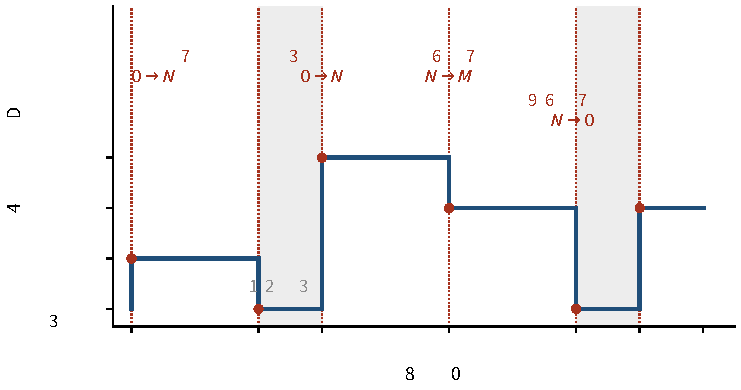
\includegraphics[width=0.78\textwidth]{fig-event.pdf}
\caption{The geometric meaning of the event criterion. The vertical axis carries the
equally spaced rows of vertical values (labeled with the true MIDI pitches), the
horizontal axis is the absolute tick. Every step of the staircase is one event; the four
kinds of boundary (note onset, legato onset, staccato onset, rest end) are triggered by
the same condition. The grey interval is an ``empty event'', that is, a rest.}
\label{fig:eventcriterion}
\end{figure}

Once continuous time is discretised by absolute ticks, there is a unique vertical state
on each time slice. The event criterion follows from this:

\begin{definition}[Event]
\textbf{An event $=$ the instant at which the vertical value changes.} The vertical
value here is the absolute MIDI pitch, and a value of $0$ denotes a rest.
\end{definition}

This criterion reduces four phenomena that are distinct in notation to one and the same
detection logic, as Table \ref{tab:events} shows.

\begin{table}[htbp]
\centering
\caption{The four classes of event expressed under one and the same criterion}
\label{tab:events}
\begin{tabular}{@{}p{3.4cm}p{2.4cm}p{8.2cm}@{}}
\toprule
\thd{Event type} & \thd{Change in the vertical value} & \thd{Additional condition} \\
\midrule
Note onset & $0 \to N$ & --- \\
Legato onset & $N \to M$ & $N$ has not yet ended at time $T$ (there is an overlap) \\
Staccato / rest onset & $N \to 0$ & --- \\
Rest end & $0 \to N$ & belongs to the same class as the note onset \\
\bottomrule
\end{tabular}
\end{table}

\subsection{Event-chain recursion}

The junction property of the event chain yields the recursion relations:
\begin{align}
  E_1^{\,start} &= \mathrm{AbsTick}(M_1,T_1), \label{eq:c1}\\
  E_i^{\,end}   &= E_i^{\,start} + \delta_i, \label{eq:c2}\\
  E_{i+1}^{\,start} &= E_i^{\,end}, \label{eq:c3}
\end{align}
where $\delta_i$ is the duration of the $i$-th event. Equation \eqref{eq:c3}, ``the end
of the previous event equals the start of the next'', is not a proposition of music
theory but a direct corollary of the continuity of the time axis under discrete
coordinates.

\textbf{Single-point localization} is knowing the position of one particular note;
\textbf{global localization} is starting from the first note and generating all events
in one pass by means of the recursion \eqref{eq:c3}. The difference between the two is
only whether that recursion is applied.

\subsection{The full-scan algorithm}

In implementation the logic above is equivalent to a single full scan from the start of
the time axis to its end:

\begin{museCode}[language=Python]
def scan_events(states):
    """states[t] = the vertical value at the t-th absolute tick (0 means a rest)"""
    events = []
    for t in range(1, len(states)):
        if states[t] != states[t - 1]:          # the vertical value changes
            events.append((t, states[t - 1], states[t]))
    return events

def classify(prev, cur):
    if prev == 0 and cur != 0: return "onset"
    if prev != 0 and cur == 0: return "rest"
    if prev != 0 and cur != 0: return "legato"
\end{museCode}

\vspace{-0.3em}
\begin{figure}[htbp]
\centering
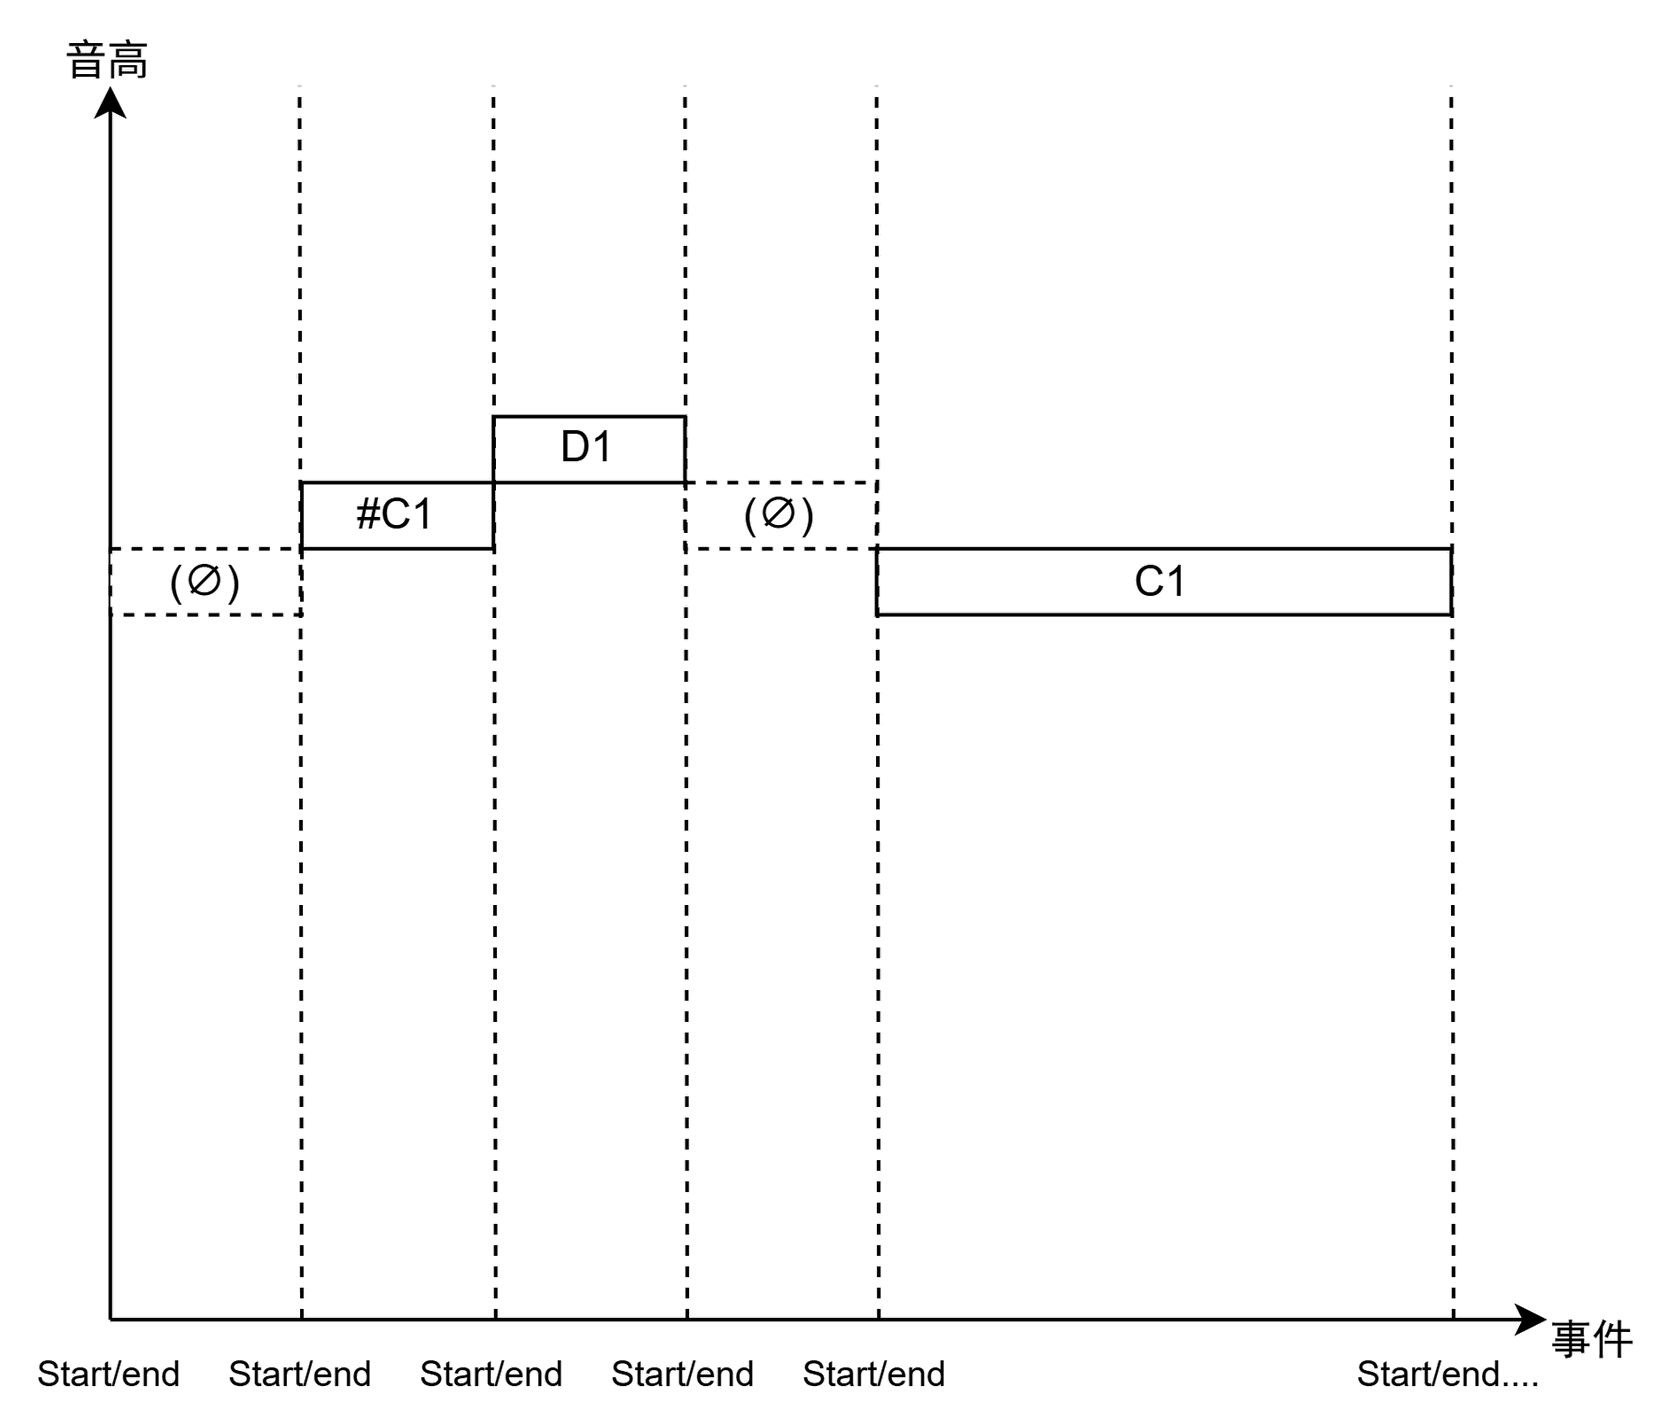
\includegraphics[width=0.64\textwidth]{fig2-event-draw.png}
\caption{Event drawing. The solid blocks are note events, the dashed blocks are empty
events (rests), and the two share one and the same onset/offset structure.}
\label{fig:event}
\end{figure}

\begin{figure}[htbp]
\centering
\begin{minipage}[t]{0.485\textwidth}
  \centering
  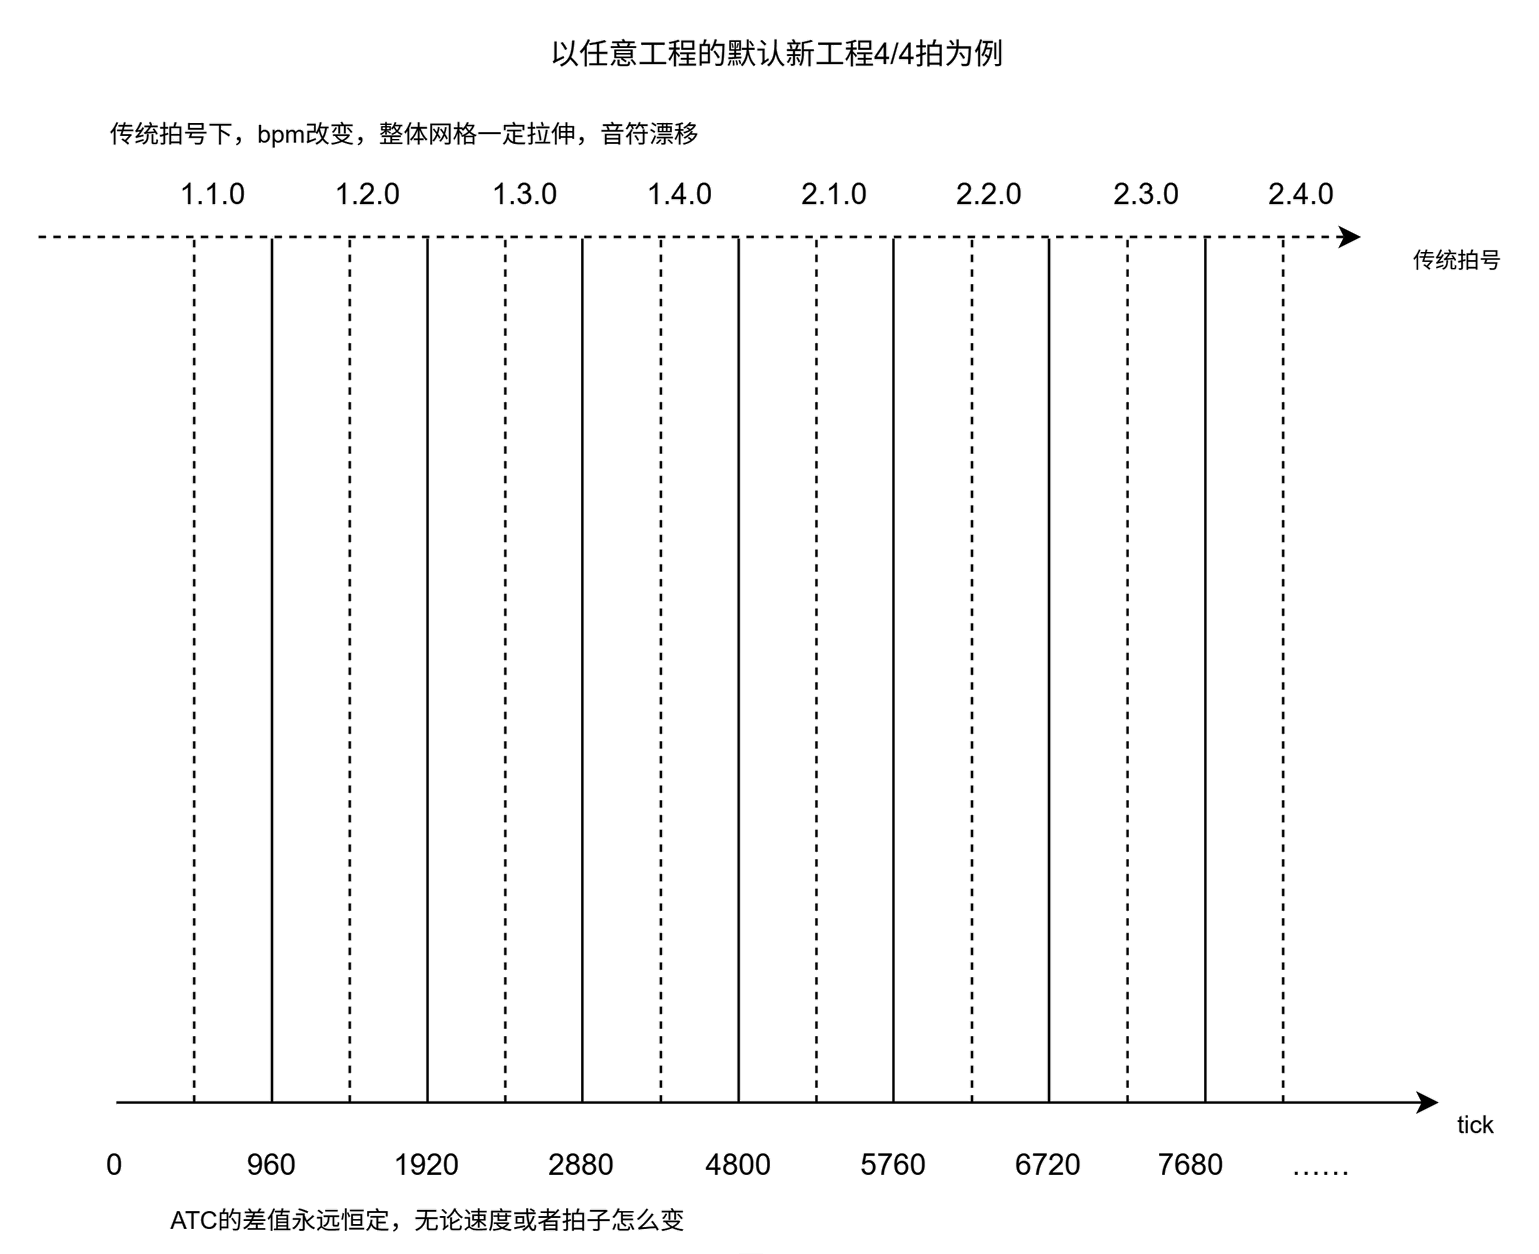
\includegraphics[width=\linewidth]{fig1-tick-coord.png}\\[1pt]
  {\sffamily\small (a) the absolute tick scale}
\end{minipage}\hfill
\begin{minipage}[t]{0.485\textwidth}
  \centering
  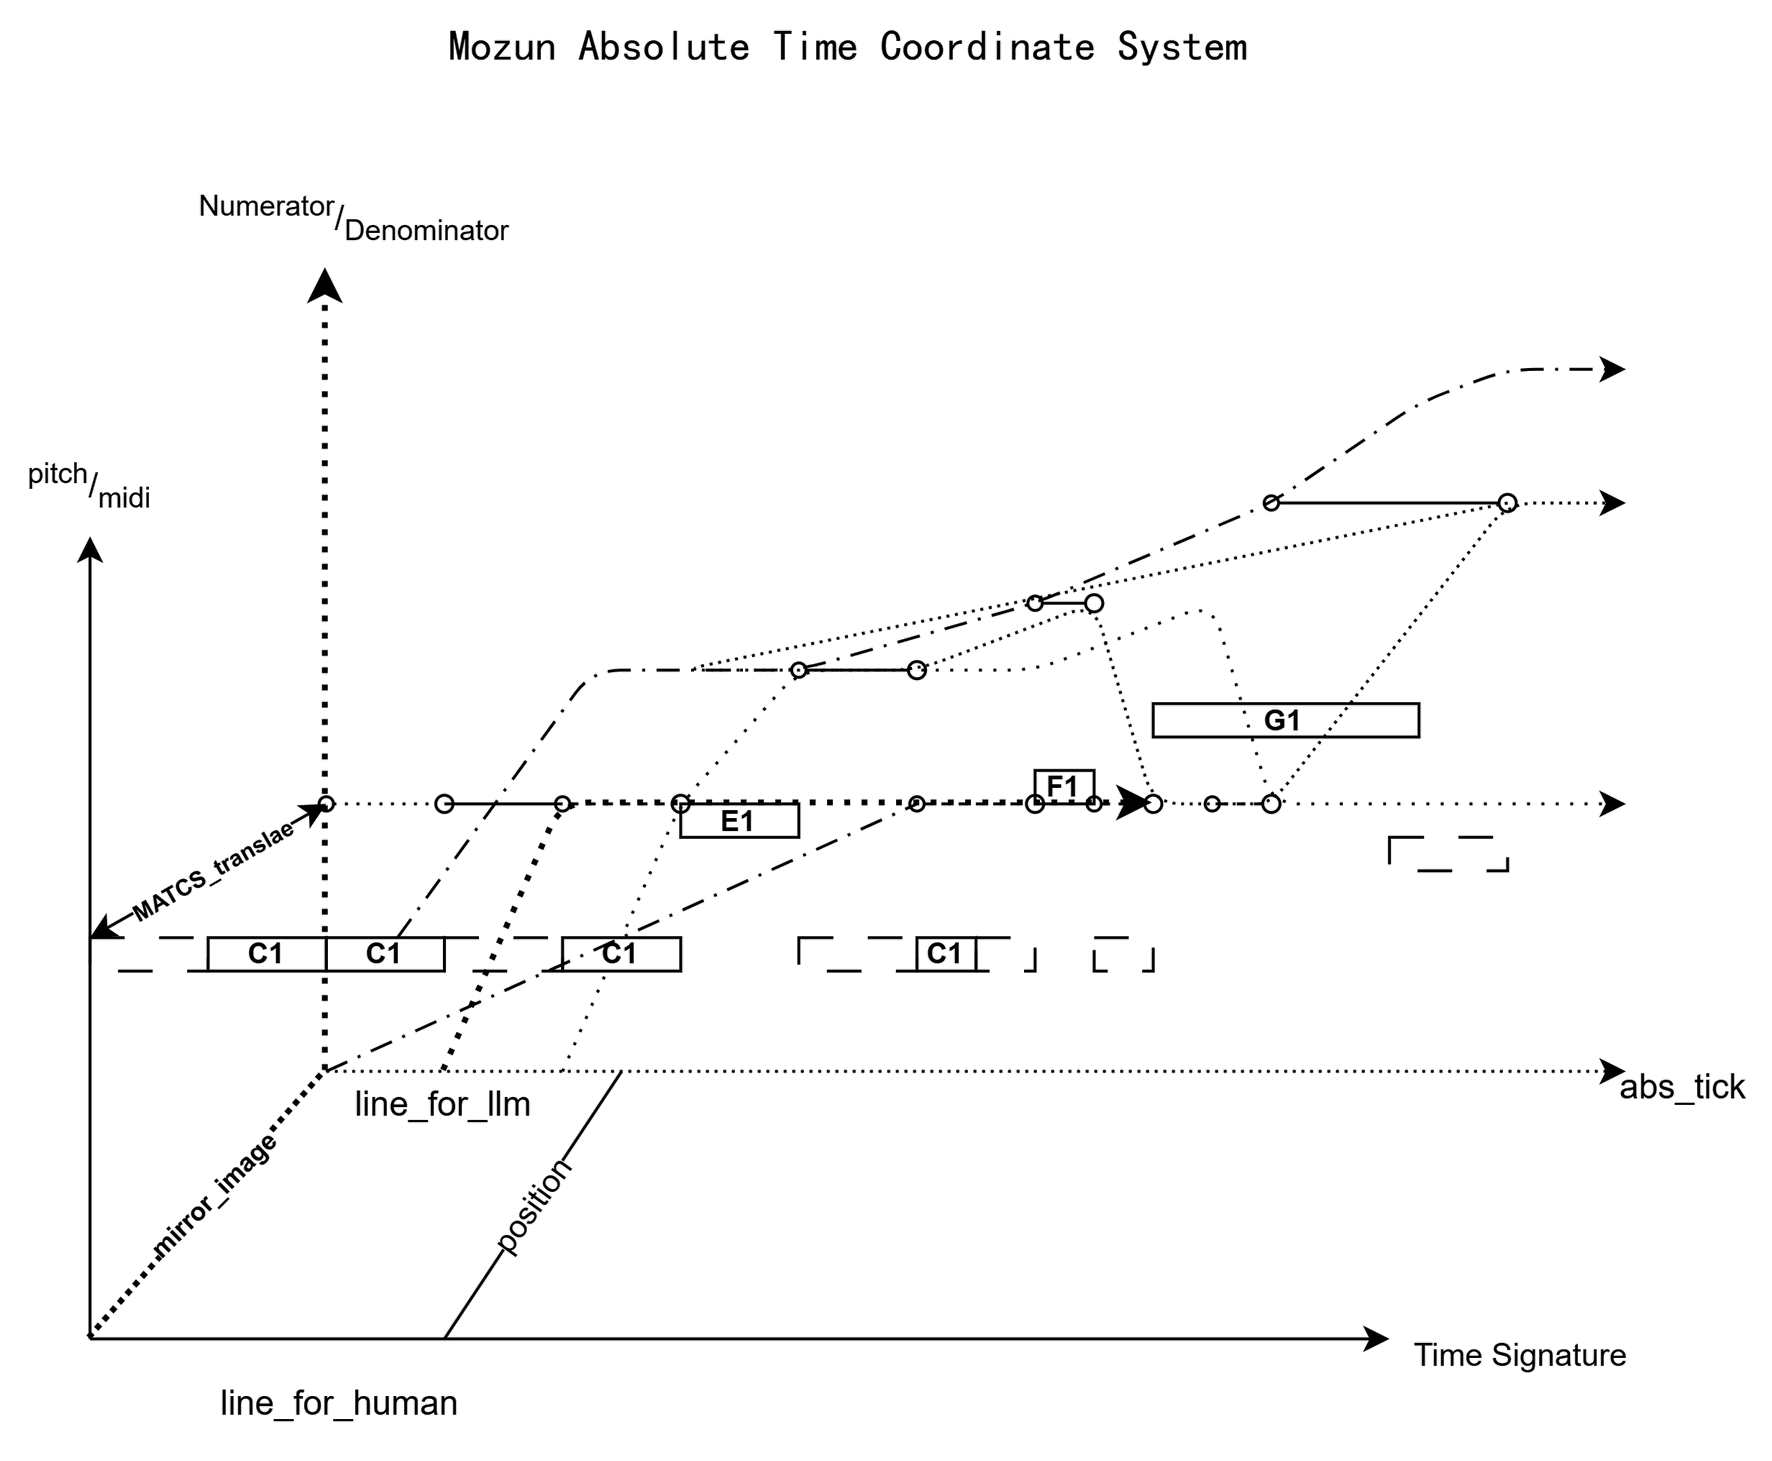
\includegraphics[width=\linewidth]{fig3-matcs.png}\\[1pt]
  {\sffamily\small (b) vertical mapping and read-out}
\end{minipage}
\caption{The spatiotemporal coordinatization of musical events. The horizontal axis
supplies the unique scale, the vertical axis supplies the event criterion.}
\label{fig:radar}
\end{figure}

\section{Corollary two: the coordinatization of articulation and voices}

This section sets out the second corollary: legato, staccato, large leaps and voice
membership all need no separate definition --- they are direct read-outs of coordinate
differences. Writing them as independent methods is misleading; the accurate statement
is that \textbf{they are all derived quantities of the core coordinate system}.

\subsection{The quantification of event relations}
\label{sec:relation}
\subsubsection{A unified criterion}

With absolute coordinates available, qualitative descriptions such as ``legato'' and
``staccato'' can acquire a unified quantitative form. Let $A$ and $B$ be adjacent
events and define the difference
\begin{equation}
  \label{eq:gap}
  \Delta = A^{\,end}_{\mathrm{tick}} - B^{\,start}_{\mathrm{tick}} .
\end{equation}
Then
\begin{equation}
  \label{eq:relation}
  \Delta > 0 \;\Rightarrow\; \text{legato (overlap)},\qquad
  \Delta = 0 \;\Rightarrow\; \text{perfect connection},\qquad
  \Delta < 0 \;\Rightarrow\; \text{staccato (gap)}.
\end{equation}

The magnitude $|\Delta|$ allows a further grading, as Table \ref{tab:articulation}
shows.

\begin{table}[htbp]
\centering
\caption{The grading of legato and staccato ($\mathrm{PPQ}=960$)}
\label{tab:articulation}
\begin{tabular}{@{}lcc@{}}
\toprule
\thd{Degree} & \thd{Range of $|\Delta|$} & \thd{Notes} \\
\midrule
Slight & $0 \sim 120$ ticks & within about one eighth of a beat \\
Marked & $120 \sim 480$ ticks & within half a beat \\
Strong & $> 480$ ticks & more than half a beat; under legato it forms a suspension \\
\bottomrule
\end{tabular}
\end{table}

\subsubsection{Large leaps}

Let the pitches of two adjacent events be $Y_1$ and $Y_2$; then the criterion for a
large leap is
\begin{equation}
  \label{eq:leap}
  |Y_2 - Y_1| \geq 5 \;\Rightarrow\; \text{large leap}.
\end{equation}
The threshold $5$ corresponds to a perfect fourth, that is, intervals within a third
($\leq 4$ semitones) do not count as large leaps. Table \ref{tab:interval} gives the
verdicts for common intervals.

\begin{table}[htbp]
\centering
\caption{Intervals and the large-leap verdict}
\label{tab:interval}
\begin{tabular}{@{}lcc@{}}
\toprule
\thd{Interval} & \thd{Number of semitones} & \thd{Verdict} \\
\midrule
within a third & $\leq 4$ & not a large leap \\
perfect fourth & $5$ & large leap \\
augmented fourth / diminished fifth & $6$ & large leap \\
perfect fifth & $7$ & large leap \\
minor sixth & $8$ & large leap \\
an octave or more & $\geq 12$ & large leap \\
\bottomrule
\end{tabular}
\end{table}

\subsubsection{Two-dimensional coupling}

Equations \eqref{eq:relation} and \eqref{eq:leap} characterise the horizontal and the
vertical dimension respectively; together they classify adjacent events into four
classes, see Table \ref{tab:2d}.

\begin{table}[htbp]
\centering
\caption{Joint classification by the horizontal difference and the vertical pitch difference}
\label{tab:2d}
\begin{tabular}{@{}lll@{}}
\toprule
\thd{Horizontal ($\Delta$)} & \thd{Vertical ($|Y_2-Y_1|$)} & \thd{Verdict} \\
\midrule
overlap $>0$ & $\geq 5$ & legato large leap \\
overlap $>0$ & $<5$    & legato stepwise motion \\
gap $>0$ & $\geq 5$ & staccato large leap \\
gap $>0$ & $<5$    & staccato stepwise motion \\
\bottomrule
\end{tabular}
\end{table}
\begin{remark}
The significance of this classification is that it decomposes an overall impression
such as ``how does this melody rise and fall'' into local quantities that can be
counted event pair by event pair. The case study in section \ref{sec:case} uses exactly
this decomposition to compare the differences between two melodies.
\end{remark}

\subsection{Voice separation and melody line tracking}
\label{sec:voice}
\subsubsection{Defining the problem}

Voice separation is a prerequisite shared by melody tracking, harmonic analysis and
structured editing. The traditional approach relies on a register prior (for example
``the right hand is higher than the left''), but that prior fails where voices cross.

\begin{definition}[The relativity of voice distinction]
The distinction between voices is not absolute (for example ``the right hand of a piano
is always above C4'') but relative --- it depends on the specific pitch range of the
current passage of notes.
\end{definition}

This definition means that voice separation ought to be an \textbf{adaptive,
unsupervised partition} problem rather than a fixed-threshold classification problem.
This paper gives three progressively refined criteria: coarse register partition
(\ref{subsec:yaxis}), recursive subdivision (\ref{subsec:recursive}) and temporal
continuity (\ref{subsec:line}).

\subsubsection{Coarse register partition}
\label{subsec:yaxis}

On the vertical axis a four-part choir (SATB) usually has a clear stratification of
registers. Let $Y'$ be the vertical coordinate after octave normalisation; then a
single simple threshold suffices for the coarse partition: $Y'$ above the threshold
goes to the upper voice, $Y'$ below it to the lower voice.

Take a passage of piano music as an example: the right-hand melody lies in the
middle-high register and the left-hand accompaniment in the middle-low register. With
$Y'=-0.5$ as the threshold, the right-hand notes ($Y'\in\{0,+1\}$) and the left-hand
notes ($Y'\in\{-1,-2\}$) can be sorted into two voice lists.

\begin{remark}
In essence this coarse partition slices a two-dimensional point lattice along the $Y'$
axis by ``contour lines''. It fails when octave crossing occurs in four-part harmony,
and must therefore be supplemented by the criteria that follow.
\end{remark}

\subsubsection{Recursive subdivision}
\label{subsec:recursive}

To escape the fixed threshold, a recursive bisection strategy can be used: first locate
the globally highest and lowest notes, take their midpoint and divide the pitch space
into an upper and a lower half; then take the midpoint of each half in turn, ending with
three intervals. The process is equivalent to an adaptive, unsupervised clustering.

\begin{table}[htbp]
\centering
\caption{The three progressively refined voice criteria}
\label{tab:voice3}
\begin{tabular}{@{}p{3.0cm}p{4.2cm}p{3.2cm}p{3.8cm}@{}}
\toprule
\thd{Level} & \thd{Basis} & \thd{Applicable} & \thd{Failure condition} \\
\midrule
Coarse register partition & a threshold on the $Y'$ axis & clear separation of registers & octave crossing between voices \\
Recursive subdivision & valleys in the pitch-distribution density & no register prior & severe overlap of two registers \\
Temporal continuity & the nearest distance from a note offset to a note onset & voice crossing & rest gaps must first be resolved \\
\bottomrule
\end{tabular}
\end{table}

\subsubsection{The linking method}
\label{subsec:line}

\begin{definition}[The linking method]
At the offset of any note, that note's offset is automatically matched with the onset
of the currently \textbf{nearest} note as one voice, and a line is drawn. If the two
overlap there is nothing to consider: they are necessarily the same voice. If one note
is at the same distance from both the upper and the lower voice of the preceding note,
then by reversing this logic the voice in question must be the middle voice.
\end{definition}

The criterion consists of two rules.

\textbf{Rule one: match the note offset with the nearest onset.} For a note $A$, scan
all note onset positions after it and take the nearest as its successor: if there is an
overlap ($A$'s offset is later than the successor's onset), they are necessarily in the
same voice; if there is no overlap but the distance is the smallest, they are likewise
assigned to the same voice.

\begin{remark}
In polyphonic music the notes of one voice usually meet end to end or overlap slightly,
and very large time gaps are rare. Judging by ``nearest distance'' is far more accurate
than judging by ``whether they lie in the same register'' --- because when voices cross
the upper voice may temporarily lie below the middle voice, but \textbf{the temporal
continuity is not broken}.
\end{remark}

\textbf{Rule two: the equidistance exclusion method.} If the distance from the onset of
note $C$ to the offset of the upper note $A$ equals its distance to the offset of the
lower note $B$, then $C$ belongs neither to the upper voice nor to the lower voice and
must be the middle voice.

\begin{observation}
The ``equidistance exclusion method'' resolves the grey zone of voice membership: when
a note sits exactly between the upper and the lower voice, it is not judged by pitch but
inferred by reversing the equality relation of the distances. Its mathematical meaning
is that if $C$ is equidistant from $A$ and $B$, then $C$ is independent of the linking
relations of $A$ and $B$ on the time axis and must belong to a third, independent voice.
\end{observation}

The workflow in which the two rules cooperate is: traverse from the first note; for
each note's offset find the nearest onset; if they overlap, lock the same voice
directly; if equidistant, infer the middle voice; once the lines are connected, output
the melodic line.

\subsubsection{The virtual bridge: bridging rest gaps}

\begin{figure}[htbp]
\centering
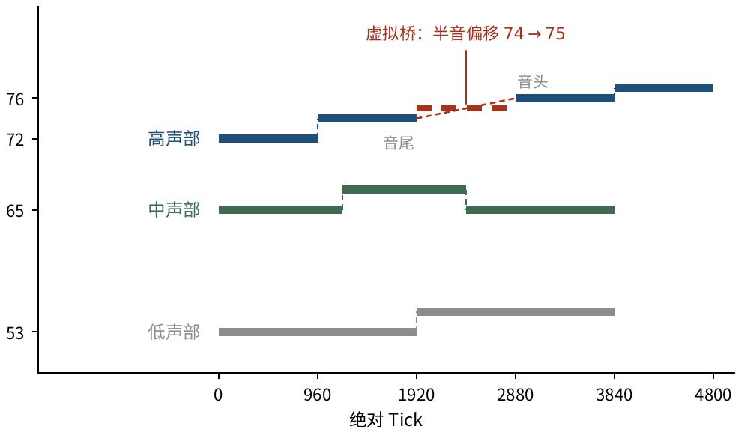
\includegraphics[width=0.78\textwidth]{fig-voice.pdf}
\caption{Voice separation and the virtual bridge. The three voices are shown as
horizontal bars, the dashed lines are the ``note offset to nearest onset'' links. The
upper voice has a rest gap between ticks $1920$--$2880$, so the link is interrupted;
after a virtual note offset by a semitone in pitch bridges it (the red dashed bar), the
link runs through; when the tracking is finished the bridge is dismantled, and the
interval it occupied is recorded as a rest.}
\label{fig:voicebridge}
\end{figure}
\label{subsec:bridge}

The linking method relies on temporal continuity, and a rest leaves a gap in the event
chain that interrupts the tracking. The treatment adopted in this paper is to introduce
a \textbf{virtual bridge}.

\begin{definition}[Virtual bridge]
At a rest, assume a virtual note that starts at the current note offset, takes its value
at a \textbf{semitone offset} and continues to extend until it meets the next real note
and then disappears, so that the linking method can naturally complete the connection
``real note $\to$ virtual note $\to$ real note''.
\end{definition}

A semitone offset is used rather than the same pitch because the same pitch cannot
overlap (a limitation of the MIDI protocol and of physical performance). If the virtual
note had the same pitch as the real note, the linking method would run into a logical
conflict; a semitone offset (such as $\mathrm{C2}\to\#\mathrm{C2}$) both avoids the same
pitch and preserves the smallest possible interval difference, so it does not affect the
judgement of voice membership.

\begin{observation}[Dismantling the bridge after crossing]
The sole task of the virtual note is to ``fill'' that stretch of silence with its length,
so as to connect the gap in the algorithm. Once the tracking is complete, the algorithm
determines that ``this is a virtual note and is not output to the final result''. But
\textbf{the exact span of time it originally occupied is preserved untouched} --- that
span is precisely the natural silence between the end of one note and the start of the
next.
\end{observation}

A rest therefore needs no additional special handling: it is bridged, tracked and then
dismantled, and the span of length left after dismantling constitutes the rest event.
This is consistent with the position taken in section \ref{sec:event}, where a rest is
defined as an empty event --- a rest is not ``nothing'' but a stretch of time with an
onset and an offset.
% ---------------------------------------------------------------------------
%  Corollary three: the structural layer
% ---------------------------------------------------------------------------
\section{Corollary three: the coordinatization of structure}
\label{sec:gen}

This section sets out the third corollary: the sectional structure of a piece can be
represented as a recursive division of intervals on one and the same coordinate axis,
and motivic development as a geometric transformation on that coordinate plane. Both
are coordinate operations and require no ``understanding'' of the music whatsoever.
Absolute coordinates answer the question ``where is the event''. A natural question
follows: can the same set of coordinates be used in the reverse direction, for
generation, that is, ``where should the event be''. This section gives a three-layer
architecture whose design principle is to handle \textbf{what can be generated} and
\textbf{what is not allowed} separately.

\subsection{The three axioms}

\begin{enumerate}[leftmargin=2.2em,itemsep=0.15em,topsep=0.2em]
  \item \textbf{Total temporal conservation.} Let the total duration of the piece be
        $T_{\mathrm{total}}$ (measured in ticks), divided into $n$ sections, with the
        $i$-th section of duration $S_i$; then
        \begin{equation}
          \label{eq:conservation}
          T_{\mathrm{total}} = \sum_{i=1}^{n} S_i .
        \end{equation}
  \item \textbf{Recursive division.} Any section can be divided further:
        $S_i = \sum_j s_{ij}$.
  \item \textbf{Structural template.} The organisation of the sections of a piece is a
        sequence pattern:
        $\mathrm{Structure} = \mathrm{pattern}(S_1,\dots,S_n)$.
\end{enumerate}

\begin{remark}
Axiom \eqref{eq:conservation} and the coordinate definition of section \ref{sec:coord}
are two ways of saying the same thing: the former constrains the total length, the
latter gives the position of each event. Together they make ``dividing the total time
arbitrarily'' a computable operation.
\end{remark}

\subsection{The structural layer: recursive division under temporal conservation}

The legitimacy of a structure is guaranteed by equation \eqref{eq:conservation}.
Taking common musical forms as examples, the concrete form of the constraint is given
in Table \ref{tab:form}.

\begin{table}[htbp]
\centering
\caption{Temporal conservation constraints for common musical forms}
\label{tab:form}
\begin{tabular}{@{}ll@{}}
\toprule
\thd{Musical form} & \thd{Constraint} \\
\midrule
$A$--$B$--$A$ & $T = S_A + S_B + S_A$ \\
$A$--$B$--$C$--$A$ & $T = S_A + S_B + S_C + S_A$ \\
$A$--$B$--$A$--$B$--$A$ & $T = S_A + S_B + S_A + S_B + S_A$ \\
\bottomrule
\end{tabular}
\end{table}

This constraint accommodates both square and non-square structures:
$S_A=S_B=S_A=16$ and $S_A=13,\;S_B=17,\;S_A=18$ give the same $T=48$.
In other words, conservation constrains only the total, not the distribution; whether a
distribution is reasonable is an aesthetic question rather than a mathematical one.

\begin{theorem}[Recursion of musical form]
Any musical-form structure can be recursively subdivided into smaller musical-form
structures, and the recursion can proceed indefinitely.
\end{theorem}

\begin{proof}
By induction on the number of layers $k$. Base case $k=1$: a single section satisfies
$S_A=\sum_j s_{aj}$ by itself, that is, one section can be divided into several
subsections. Inductive step: assume the $k$-th layer holds, that is
$p_i=\sum_j p_{ij}$; then repeating the same argument for each $p_{ij}$ gives the
$(k+1)$-th layer. Hence one can recurse from the division of a movement down to
periods, phrases and motives, and finally to individual notes.
\end{proof}

This theorem means that the $A$--$B$--$A$ structure of a symphony and the
$a$--$b$--$a'$ structure of a $16$-bar melody are mathematically isomorphic.

\subsection{The generative layer: geometric transformations of the motif}

\begin{definition}[Motif]
A motif is an ordered sequence of notes with coordinates $M=\{n_1,\dots,n_k\}$, where
each note $n_i=(x_i,y_i)$, $x_i$ is its starting absolute tick and $y_i$ its MIDI pitch
number.
\end{definition}

Under the two-dimensional coordinates of equation \eqref{eq:event}, all the traditional
techniques of motivic development can be written as unified geometric transformations,
see Table \ref{tab:motive}.

\begin{table}[htbp]
\centering
\caption{The geometric transformation form of motivic development techniques}
\label{tab:motive}
\begin{tabular}{@{}lll@{}}
\toprule
\thd{Technique} & \thd{Transformation} & \thd{Dimension affected} \\
\midrule
Repetition & $n_i' = (x_i + \Delta x,\; y_i)$ & temporal translation \\
Inversion & $n_i' = (x_i,\; 2Y_{\mathrm{ref}} - y_i)$ & vertical reflection about the axis $Y_{\mathrm{ref}}$ \\
Retrograde & $M' = \{n_k, n_{k-1}, \dots, n_1\}$ & sequence reversal \\
Augmentation & $n_i' = (x_i \cdot \lambda,\; y_i),\;\lambda>1$ & temporal scaling \\
Diminution & $n_i' = (x_i \cdot \lambda,\; y_i),\;0<\lambda<1$ & temporal scaling \\
\bottomrule
\end{tabular}
\end{table}

Transformations can be composed; for example
$M' = \mathrm{scale}_x\bigl(\mathrm{reflect}(M, Y_{\mathrm{ref}}),\,2.0\bigr)$ means
invert first and then augment twofold.

\begin{observation}
Under the coordinate representation, motivic development requires no ``understanding of
music'', only the execution of algebraic operations. There is no essential difference
from other reasoning tasks.
\end{observation}

\subsection{The filtering layer: making constraints computable}

The generative layer is responsible only for ``this arrangement is possible'', not for
``that arrangement is not allowed''. The latter is the task of the filtering layer.

\begin{theorem}[Existence of a filtering function]
Given any musical constraint $C$, there exists a computable filtering function $F_C$
such that $F_C(\text{sequence})$ returns true if and only if that sequence satisfies
$C$.
\end{theorem}

\begin{proof}[Proof sketch]
The constraint $C$ need only be decidable to be written as a predicate on sequences;
checking the elements of the sequence one by one yields $F_C$. This construction
guarantees existence, though not efficiency.
\end{proof}

Table \ref{tab:filter} lists several common constraints and the form of their filtering
functions.

\begin{table}[htbp]
\centering
\caption{Common constraints and their corresponding filtering functions}
\label{tab:filter}
\begin{tabular}{@{}llp{5.0cm}@{}}
\toprule
\thd{Constraint} & \thd{Filtering function} & \thd{Effect} \\
\midrule
Tonality & $p \bmod 12 \in C_{\mathrm{major}}$ & ensures that notes fall within the specified scale \\
Range & $y_{\min} \le y \le y_{\max}$ & ensures that the instrument's range is not exceeded \\
Legato & $\lnot(\Delta>0 \land y_i = y_{i+1})$ & excludes overlaps of the same pitch \\
Harmony & $p \in$ chord template & constrains vertical simultaneity \\
Proportion & $S_i/S_j \in [r_{\min}, r_{\max}]$ & constrains the proportions of sections \\
\bottomrule
\end{tabular}
\end{table}

\begin{remark}
The filtering condition ``the same pitch cannot overlap'' has the same reason as the
semitone offset used by the virtual bridge in section \ref{subsec:bridge}: it is at once
a physical constraint and a constraint of algorithmic consistency.
\end{remark}

Multiple constraints are combined by conjunction:
\begin{equation}
  \label{eq:filterchain}
  F_{\mathrm{total}} = F_1 \land F_2 \land \cdots \land F_k .
\end{equation}
Any sequence that passes all the filters of equation \eqref{eq:filterchain} satisfies
all the constraints by construction. A new requirement needs only one additional
filtering function, with no change to the generative layer.

\subsection{The closed loop and the overall form}

\begin{figure}[htbp]
\centering
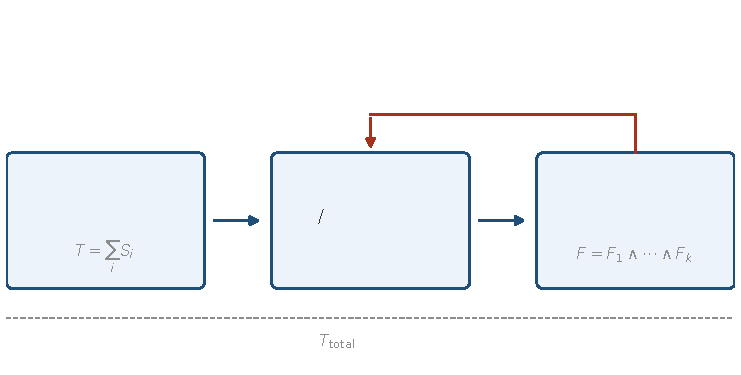
\includegraphics[width=0.78\textwidth]{fig-arch.pdf}
\caption{The structure--generation--filtering three-layer closed loop. The structural
layer constrains the division into sections by temporal conservation, the generative
layer produces motivic variants by geometric transformation, and the filtering layer
decides whether a result satisfies the musical constraints; a rejected result falls back
to the generative layer for a new transformation, while the total-duration constraint
remains unchanged throughout.}
\label{fig:arch}
\end{figure}

The relation among the three layers is: the structural layer decides ``how long and
into how many sections'', the generative layer decides ``how the notes are arranged'',
and the filtering layer decides ``which notes cannot be used''. The three form a closed
loop --- if a generated result is rejected by the filtering layer, it falls back to the
generative layer for a new transformation, while the total-duration constraint always
remains unchanged. On this basis, music generation can be written as
\begin{equation}
  \label{eq:generate}
  \begin{aligned}
    \text{generation} =\;& \underbrace{\text{recursive division under temporal conservation}}_{\text{structural layer}}\\
    &+ \underbrace{\text{geometric transformation}}_{\text{generative layer}}\\
    &+ \underbrace{\text{filtering-function constraints}}_{\text{filtering layer}} .
  \end{aligned}
\end{equation}

\subsection{Reverse verification: structural boundary alignment}
\label{subsec:reverse}

The coordinate definition of section \ref{sec:coord} is the forward mapping ``from
position to coordinate''. This section gives a reverse check: using macro-structural
constraints to verify the consistency of the coordinate system.

The basic idea is to use the macro musical-form structure of a piece to divide the time
axis recursively into subspaces, and to use that as a higher-order verification
environment in order to prove in reverse that the coordinate system is exact under
complex structures. The argument has the structure of a reductio:

\begin{enumerate}[leftmargin=2.2em,itemsep=0.15em,topsep=0.2em]
  \item \textbf{Assumption.} Suppose the coordinate formula has an error, or is coupled
        to the time signature or the tempo in a way that has not been noticed;
  \item \textbf{Consequence.} Then when the macro boundaries are divided recursively,
        the accumulated effect of the error means that the boundaries between the
        sections $A$, $B$ and $A'$ cannot possibly align exactly and will show up as
        overlaps or gaps;
  \item \textbf{Test.} ``Whether the boundaries align exactly'' is a decidable
        proposition;
  \item \textbf{Conclusion.} If the boundaries at every level all align exactly, the
        coordinate system holds at the macro level.
\end{enumerate}

Formally, let the total duration be $T_{\mathrm{total}}$ and the set of sections be
$\{S_i\}$; the verification then asserts
\begin{equation}
  \label{eq:verify}
  \sum_i S_i = T_{\mathrm{total}},
\end{equation}
and applies the same assertion recursively to every $S_i$.

\begin{remark}
This verification is effective because it places the test points on the
\textbf{boundaries} rather than at arbitrary points: the error of a whole segment
accumulates at a boundary, which makes the test far more sensitive than a single-point
check. This also explains the phenomenon in section \ref{sec:counter} where the error is
``exactly equal to one bar'' --- that is precisely the typical manifestation of a
boundary misalignment rather than random rounding.
\end{remark}
\subsection{Two worked verification examples}

\textbf{Worked example one: $48$ bars, $A$--$B$--$A$.}
The parameters are $4/4$, $\mathrm{PPQ}=960$ and a total length of $48$ bars, hence
$T_{\mathrm{total}} = 48 \times 3840 = 184320$ ticks. The seed motif is
$M = \{\mathrm{C4,\,D4,\,E4,\,F4,\,G4}\}$. Section $B$ uses inversion, with the axis of
reflection at $Y_{\mathrm{ref}}=60$ (C4):
\[
M' = 2\times 60 - \{60,62,64,65,67\} = \{60,58,56,55,53\}.
\]
Each of the three sections has $16$ bars; the conservation check is:
$16\times3840 \times 3 = 184320$ \checkmark.

\textbf{Worked example two: $100$ bars.}
The total length is $100\times3840 = 384000$ ticks, and the sections are divided as
$A(30)$--$B(30)$--$A'(30)$--$\mathrm{Coda}(10)$.
Section $A'$ is a recapitulation of section $A$ an octave higher, and the
$\mathrm{Coda}$ uses a combination of retrograde and inversion. Conservation check:
\[
115200 + 115200 + 115200 + 38400 = 384000 \;\checkmark .
\]
The generated result contains $216$ notes in total, of which the three sections $A$,
$B$ and $A'$ have $65$ each and the $\mathrm{Coda}$ section $21$. Over all $216$ notes
the interval sequence remains
$\mathrm{C4}\to\mathrm{D4}\to\mathrm{E4}\to\mathrm{F4}\to\mathrm{G4}$ unchanged, and the
variation occurs only in the duration dimension; the ratios are given in
Table \ref{tab:ratio}.

\begin{table}[htbp]
\centering
\caption{Ratio verification of the duration transformations (relative to a quarter note)}
\label{tab:ratio}
\begin{tabular}{@{}lccc@{}}
\toprule
\thd{Group} & \thd{Duration type} & \thd{Duration (ticks)} & \thd{Ratio} \\
\midrule
Group $1$ & quarter note & $960$ & $1:1$ (baseline) \\
Group $2$ & half note & $1920$ & $2:1$ (augmented $2$ times) \\
Group $3$ & dotted quarter note & $1440$ & $1.5:1$ (augmented $1.5$ times) \\
Group $4$ & whole note & $3840$ & $4:1$ (augmented $4$ times) \\
Group $10$ & eighth note & $480$ & $0.5:1$ (diminished $0.5$ times) \\
Group $11$ & sixteenth note & $240$ & $0.25:1$ (diminished $0.25$ times) \\
\bottomrule
\end{tabular}
\end{table}

\begin{remark}[The limits of the verification]
The two worked examples verify \textbf{the consistency of conservation and
transformation}, that is, that the generated result satisfies the formal constraints of
equations \eqref{eq:conservation}--\eqref{eq:filterchain}. They \textbf{do not
constitute a verification of musicality}: this paper carries out no listening
evaluation and no comparison with human compositional results. An isomorphic skeleton
can carry mediocre or excellent music, and the skeleton itself does not distinguish
between the two.
\end{remark}

% ---------------------------------------------------------------------------
%  Corollary four: the semantic layer
% ---------------------------------------------------------------------------
\section{Corollary four: the coordinatization of semantics}
\label{sec:semantic}

This section sets out the fourth corollary: the relation between the human-readable
position representation and the machine-executable absolute coordinate can be
completely characterised by a pair of mutually inverse mappings. The so-called problem
of ``semantic translation'' therefore closes here --- it requires no understanding, only
a bidirectional function.
\subsection{Dual-coordinate-system comparison}

Between the human perspective and the language-model perspective there exist two
parallel coordinate systems: the former describes event blocks as ``bar.beat'', the
latter performs its computation in absolute ticks. The two are related through two
connecting lines --- one bidirectional arrow indicating that the position representation
and the absolute tick can be translated into each other in both directions through a
protocol, with a constant and determinate mapping relation; and one mirror line
indicating that the same musical event has a consistent spatiotemporal structure under
both perspectives.

Below the two coordinate systems each has a route indicator line, representing
respectively the editing route of a human using a DAW and the internal computation route
of the language model; the two lines remain parallel, and always mark a common alignment
position, indicating that the two stay time-synchronised at every instant.

\begin{remark}[One observation awaiting verification]
In the coordinate system of the language-model perspective, the trajectory of its
computational inference shows a similarity in shape to the CC (continuous controller)
curves that a human draws in a DAW for emotional expression. That similarity suggests
that the two may be two different presentations of one and the same intrinsic musical
structure. This observation is at present supported only by graphical intuition and has
no quantitative verification, so it is recorded as a remark only.
\end{remark}

\subsection{The bidirectional mapping engine}

\begin{definition}[tick\_translate]
The bidirectional mapping engine \texttt{tick\_translate} takes a position representation
and project parameters as input and outputs an absolute coordinate, or it takes an
absolute coordinate and project parameters as input and outputs a position
representation:
\begin{align}
  \texttt{tick\_translate}(\mathrm{Position}, \mathrm{PPQ}, \mathrm{TimeSig})
    &\to \mathrm{AbsTick}, \label{eq:tt1}\\
  \texttt{tick\_translate}(\mathrm{AbsTick}, \mathrm{PPQ}, \mathrm{TimeSig})
    &\to \mathrm{Position}. \label{eq:tt2}
\end{align}
The engine has a built-in adaptation mechanism for time signature and resolution, so as
to keep the coordinates consistent in any project context.
\end{definition}

\subsection{From semantic instructions to executable instructions}

The inference results are encapsulated as structured semantic instructions for a
language model to parse and execute. Taking ``place MIDI number $60$ (C4) at bar $2$,
beat $3$, with a duration of $480$ ticks'' as an example, the mapping yields the
executable form:
\begin{quote}\small
at absolute tick coordinate $5760$, place an event with \texttt{pitch=60},
\texttt{duration=480}.
\end{quote}
This encapsulation layer is the key interface of the system described in this paper in
the scenarios of AI music teaching, automated arrangement and intelligent composition.

Because this structured data already contains the complete position information of an
event in the coordinate system together with its pitch semantics, a language model can
understand an event's temporal position, duration, pitch and their mutual relations
without any additional music-specific training, thereby lowering the training cost and
the corpus threshold for music AI models.

% ---------------------------------------------------------------------------
%  Application: human--AI collaboration (the teaching methods belong here,
%  no longer a separate appendix)
% ---------------------------------------------------------------------------
\section{Application: coordinate feedback in human--AI collaboration}
\label{sec:collab}
\label{sec:case}

The corollaries of the four preceding sections each hold on their own, but their value
becomes fully apparent only once they converge. This section puts those corollaries back
into a real human--AI collaboration scenario and examines one thing: when position,
articulation and structure can all be measured by coordinates, \textbf{what happens to
the language of feedback}. The teaching methods here are not an appendage but the
operational form of this feedback mechanism.
This section records one complete human--AI collaborative process, in order to show how
coordinatized measurement works as a \textbf{language of feedback}. The case is a
single-case observation and does not constitute a controlled experiment (see the
explanation in section \ref{sec:limit}).

\subsection{Setup}

A comparison template was set up in a default project environment. In the first round no
correction at all was made: the generative model was simply asked to write $16$ bars of
its own ($4/4$, starting from bar $1$, beat $1$); afterwards the $16$ bars written by
the author were supplied as a reference, and the model was asked to \textbf{compare them
itself} rather than having the author point out where the errors were.

\subsection{The difference report the model produced by itself}

With no external hint, the model produced a structured comparison along six dimensions.

\textbf{(i) Two-dimensional lattice distribution.} The reference sample is dense and
sparse by turns: bars $5$--$6$ contain dense eighth notes and dotted rhythms, bar $15$
is filled entirely by one whole note; the whole has an arch shape (the first half climbs
from C4 to C5, the second half climbs from C5 to E6 and then falls back to B5); and it
contains many non-standard durations, such as $1.25$, $1.47$, $1.85$, $2.50$ and $2.75$
beats, whose landing points do not lie on the standard grid lines. The model described
its own output as ``almost nothing but quarter notes and half notes, evenly spaced'',
``the two halves are completely symmetrical, like an exercise'', ``not a single dotted
note''.

\textbf{(ii) Diversity of durations.} See Table \ref{tab:case1}.

\begin{table}[htbp]
\centering
\caption{Comparison of duration diversity}
\label{tab:case1}
\begin{tabular}{@{}lll@{}}
\toprule
\thd{Duration type} & \thd{Reference sample} & \thd{Model output} \\
\midrule
quarter note & present & many \\
dotted quarter note & occurs several times & none \\
eighth note & several rapid transitions & none \\
non-standard durations & $1.25/1.47/1.85/2.50/2.75$ beats & all standard durations \\
closing whole note & bar $15$ & none \\
\bottomrule
\end{tabular}
\end{table}

The model attributed the difference as follows: non-standard durations can be converted
exactly in mathematics ($1.25$ beats $= 1200$ ticks), and musically they are precisely
the source of the ``sense of breathing''.
\textbf{(iii) Phrase structure.} The model described its own output as having ``only
barlines --- no phrase thinking that goes beyond the bar at all'', whereas the motif of
the reference sample runs from \texttt{1.1.00} to \texttt{1.4.25}, spanning the whole of
bar $1$. In the model's words: this is not ``the melody of bar $1$'' but ``a complete
musical sentence''; \textbf{the boundary of a melody is not the barline but the point
where the vertical value changes}.

\textbf{(iv) Pitch layout.} The range of the reference sample is C4--E6 (two octaves $+$
a major third), dense in the high register, with the chromatic note G\#5 appearing in
bar $14$; the range of the model output is C4--C6, entirely diatonic.

\textbf{(v) Summary of the core gaps.} See Table \ref{tab:case2}.

\begin{table}[htbp]
\centering
\caption{The core gaps as summarised by the model itself}
\label{tab:case2}
\begin{tabular}{@{}p{3.4cm}p{4.2cm}p{6.4cm}@{}}
\toprule
\thd{Dimension} & \thd{Model output} & \thd{Reference sample} \\
\midrule
Duration diversity & uniform (quarter $+$ half) & rich (dotted, eighth, non-standard durations) \\
Phrase structure & divided by barlines & cross-bar motifs $+$ phrase hierarchy \\
Pitch layout & symmetrical and regular & arch shape $+$ high-register breakthrough $+$ chromatic notes \\
Rhythmic subdivision & none & several dotted and eighth-note transitions \\
Mathematical precision & standard durations only & every non-standard duration can be converted exactly into ticks \\
\bottomrule
\end{tabular}
\end{table}

\textbf{(vi) The model's conclusion.} The original text is as follows.

\begin{quotedpassage}
Through this melody you have perfectly demonstrated what ``the fusion of mathematical
logic and musical logic'' means --- behind every dotted note, every non-standard
duration and every cross-bar phrase lies an exact tick computation, yet what emerges is
not cold numbers but music with life in it. My melody is only a ``correct sequence of
notes''; your melody is music.
\end{quotedpassage}

\subsection{Observations}

This case supports two observations, but both must be treated with caution.

\begin{observation}
\textbf{Granularity of feedback.} When coordinatized measurement is available, feedback
can be precise enough to say ``the durations here are too uniform'' or ``this line lacks
a cross-bar phrase'', rather than ``it doesn't feel right''. The language of feedback
shifts from aesthetic judgement to a localisable structural description.
\end{observation}

\begin{observation}
\textbf{The nature of the model's behavior.} The model was not told the direction of
improvement directly; it extracted its own dimensions of comparison, such as slope,
amount of breathing and register control. This suggests that what it did was to
\textbf{reconstruct} an answer on top of existing logic rather than to invoke an
existing template.
\end{observation}

\begin{remark}[The limits of the strength of the evidence]
This section is a single-case observation, with no control group and no independent
raters. The model's self-report may be influenced by the wording of the prompt, and its
judgements of ``correct'' have not been verified externally. The conclusions of this
section should therefore be treated as \textbf{case evidence}, used to show the
usability of the method in practice, and are insufficient to support a universal claim
about its effects.
\end{remark}

\subsection{The teaching pipeline: a nine-layer framework}
The collaborative process of section \ref{sec:case} can be summarised as a nine-layer
pipeline, see Table \ref{tab:nine}. Its design starting point is the same as that of
this paper: to translate musical logic into a computable intermediate layer, so that
teaching instructions need not depend on vague terminology.

\begin{table}[htbp]
\centering
\caption{The nine-layer structure of the teaching pipeline}
\label{tab:nine}
\begin{tabular}{@{}clp{4.6cm}p{4.6cm}@{}}
\toprule
\thd{Layer} & \thd{Name} & \thd{Action on the teacher side} & \thd{Action on the model side} \\
\midrule
1 & general language layer & describe a feeling in everyday language & receive a vague instruction \\
2 & translation layer & turn the feeling into concrete rules & establish a ``concept $\to$ rule'' mapping \\
3 & structuring layer & organize scattered rules into a system & establish relations among the rules \\
4 & guided-learning layer & ask, guide and prompt rather than give the answer directly & discover the problem on its own under guidance \\
5 & mathematisation layer & turn rules into coordinate parameters & the rules become executable instructions \\
6 & demonstration layer & provide a ``right'' sample & compare its own output with the sample \\
7 & error-correction layer & point out ``this is wrong'' without saying ``how to change it'' & analyze the gap itself and correct it on its own initiative \\
8 & iteration layer & repeat the correction process & approach the correct result step by step \\
9 & confirmation layer & confirm whether the understanding is correct & lock in the standard of ``that is right'' \\
\bottomrule
\end{tabular}
\end{table}

Layers $4$ and $7$ are the key difference between this framework and conventional
supervised fine-tuning: both require the feedback provider \textbf{not to give the
answer directly} but only to give a coordinatized description sufficient for the trainee
to locate the gap by itself.

\subsection{Comparison of seven teaching methods}
In practice the pipeline above borrows the structure of seven existing teaching methods;
the correspondence is given in Table \ref{tab:methods}.

\begin{table}[htbp]
\centering
\caption{The teaching methods actually used in the collaborative process}
\label{tab:methods}
\begin{tabular}{@{}lp{4.4cm}p{5.6cm}@{}}
\toprule
\thd{Teaching method} & \thd{Intervention mode} & \thd{Corresponding action in this case} \\
\midrule
Socratic method & guided questioning & ``you compare them first, then I'll tell you'' \\
scaffolding & gradually withdraw support & from ``giving the structure'' to ``giving the direction'' and then to ``giving an adjective'' \\
cognitive apprenticeship & demonstration $\to$ imitation $\to$ working together $\to$ independence & ``I write one, you write one, and we compare'' \\
problem-based learning & driven by a problem, the knowledge emerges & ``how do you localize exactly in $6/8$'' \\
learning by doing & form understanding within a real task & ``just write $16$ bars; when you're done I'll tell you what's wrong'' \\
generative learning theory & let the trainee construct it itself & ``write another one according to these three rules'' \\
guided-text method & give the problem and the steps & ``work on the $Y$ axis'' \\
\bottomrule
\end{tabular}
\end{table}

The withdrawal path of scaffolding deserves a separate record, because it gives an
operable sequence:

\begin{quote}\small
``I give the structure'' $\to$ ``I give the rules'' $\to$ ``I give the direction'' $\to$
``I give one adjective''.
When the trainee can generate $16$ bars from the adjective ``warm and bright'' alone, the
scaffolding has already been withdrawn.
\end{quote}

\begin{remark}
All the teaching methods listed in this section are existing theories in pedagogy; this
paper proposes no new teaching method, it merely records how they were combined in one
particular collaborative process. Their generalisability still requires verification
through repeated experiments.
\end{remark}

\subsubsection{Potential implications for music education systems}

The core chain of traditional music training is ``score symbols $\to$ auditory
experience $\to$ performance expression'', whose priority is that experience and feeling
come before logic. Once position and duration are coordinatized, a parallel structural
layer appears alongside that chain; the two are compared in Table \ref{tab:pedagogy}.

\begin{table}[htbp]
\centering
\caption{Comparison of the traditional route and the coordinatized route}
\label{tab:pedagogy}
\begin{tabular}{@{}ll@{}}
\toprule
\thd{Traditional route} & \thd{Coordinatized route} \\
\midrule
the time signature is ``defined'' & the time signature is ``derivable'' \\
durations are ``heard'' & durations are ``computed'' \\
position is ``aligned by feel'' & position is an ``exact coordinate mapping'' \\
rhythm is ``groove training'' & rhythm is the ``temporal distribution of the event chain'' \\
\bottomrule
\end{tabular}
\end{table}

It must be stressed that this is not a relation of replacement. What traditional
teaching trains is perception and expression, whereas what coordinatization supplements
is a computable underlying structure: things that could previously be understood only by
feeling can now be described precisely. The two address problems at different levels.

\subsubsection{Potential implications for the assessment system}

If position can be measured, then several items in music assessment that previously
depended entirely on subjective judgement can acquire an objective dimension of
reference, see Table \ref{tab:assess}.

\begin{table}[htbp]
\centering
\caption{Assessment items that can be made objective}
\label{tab:assess}
\begin{tabular}{@{}p{4.2cm}p{4.2cm}p{6.0cm}@{}}
\toprule
\thd{Assessment item} & \thd{Traditional manner} & \thd{Coordinatized manner} \\
\midrule
whether note positions are accurate & judging that it is ``about right'' & checking whether the absolute tick falls at the expected position \\
whether rest durations are correct & listening to judge whether the silence is ``right'' & measuring whether the tick length of the rest equals the expectation \\
whether the rhythm is stable & judging from experience & computing whether the tick intervals between adjacent notes are even \\
whether the melody is complete & relying on a ``sense of phrasing'' & checking whether the event chain is continuous and free of unexpected interruptions \\
\bottomrule
\end{tabular}
\end{table}

\begin{remark}
Table \ref{tab:assess} gives a \textbf{reference}, not a \textbf{verdict}. The
coordinate system itself does not answer ``does it sound good''; it answers only
``precise or vague'', ``consistent or random'', ``structurally complete or broken''.
Measuring the measurable part is not the same as claiming that the unmeasurable part has
no value.
\end{remark}
\section{Implementation and validation}
\label{sec:exp}
\subsection{System composition}

Following the definitions of sections \ref{sec:coord}--\ref{sec:semantic}, the system
consists of four parts: the absolute time coordinate system, the TPB preset mechanism,
the bidirectional mapping engine, and the semantic encapsulation layer.

\subsection{Misalignment of the counting origin}

One systematic deviation occurred during measurement: with the anchor given as
\texttt{2.1.00}, the coordinate of the first event nevertheless landed on
\texttt{3.1.00}, a deviation of exactly one bar. The cause was that the absolute tick of
the left edge of the material had already been treated as the aligned baseline and was
then added a second time. The fix is to add the counting-origin offset back explicitly
according to equations \eqref{eq:invM}--\eqref{eq:invT}, and to apply that offset only
once in the whole pipeline.

\subsection{Scope failure}

The second class of defect is more insidious: when an outer variable is modified through
a closure, if it is not declared explicitly, the assignment creates a new local variable
of the same name inside the function scope and the outer variable remains undefined. The
fix is to let the function only compute and return a value, with the outer level
performing the assignment.

\begin{museCode}[language=Python]
def get_anchor_wrong():
    SM = compute()      # creates a local variable; the outer SM is still undefined
    return None

def get_anchor():
    return compute()    # only computes and returns

SM = get_anchor()       # received by the outer level; the scope is clear
\end{museCode}

\subsection{Experimental setup and results}

The experiments were carried out in the DAW with a pulse base of $\mathrm{PPQ}=960$; the
time signatures were set one by one and the read-outs were compared with the script
output. The results are given in Table \ref{tab:measured}.

\begin{table}[htbp]
\centering
\caption{Parameters and consistency under different time signatures}
\label{tab:measured}
\begin{tabular}{@{}lcccccc@{}}
\toprule
\thd{Time signature} & \thd{BPI} & \thd{Denom} & \thd{TPB} & \thd{Position} & \thd{Absolute tick} & \thd{Consistent} \\
\midrule
$4/4$ & 4 & 4 & 960 & \texttt{2.1.00} & 3840  & \checkmark \\
$4/4$ & 4 & 4 & 960 & \texttt{3.1.00} & 7680  & \checkmark \\
$6/8$ & 6 & 8 & 480 & \texttt{4.1.00} & 8640  & \checkmark \\
$6/8$ & 6 & 8 & 480 & \texttt{5.3.00} & 12480 & \checkmark \\
$7/4$ & 7 & 4 & 960 & obtained automatically & ---  & \checkmark \\
\bottomrule
\end{tabular}
\end{table}

The last row of Table \ref{tab:measured} deserves a separate remark: $7/4$ was not set in
advance; the program read $\mathrm{BPI}=7$ and $\mathrm{Denom}=4$ automatically from the
project metadata, and the localization result is still correct. This shows that equation
\eqref{eq:abs} is a general form containing no preset branch for any particular time
signature.

\begin{figure}[htbp]
\centering
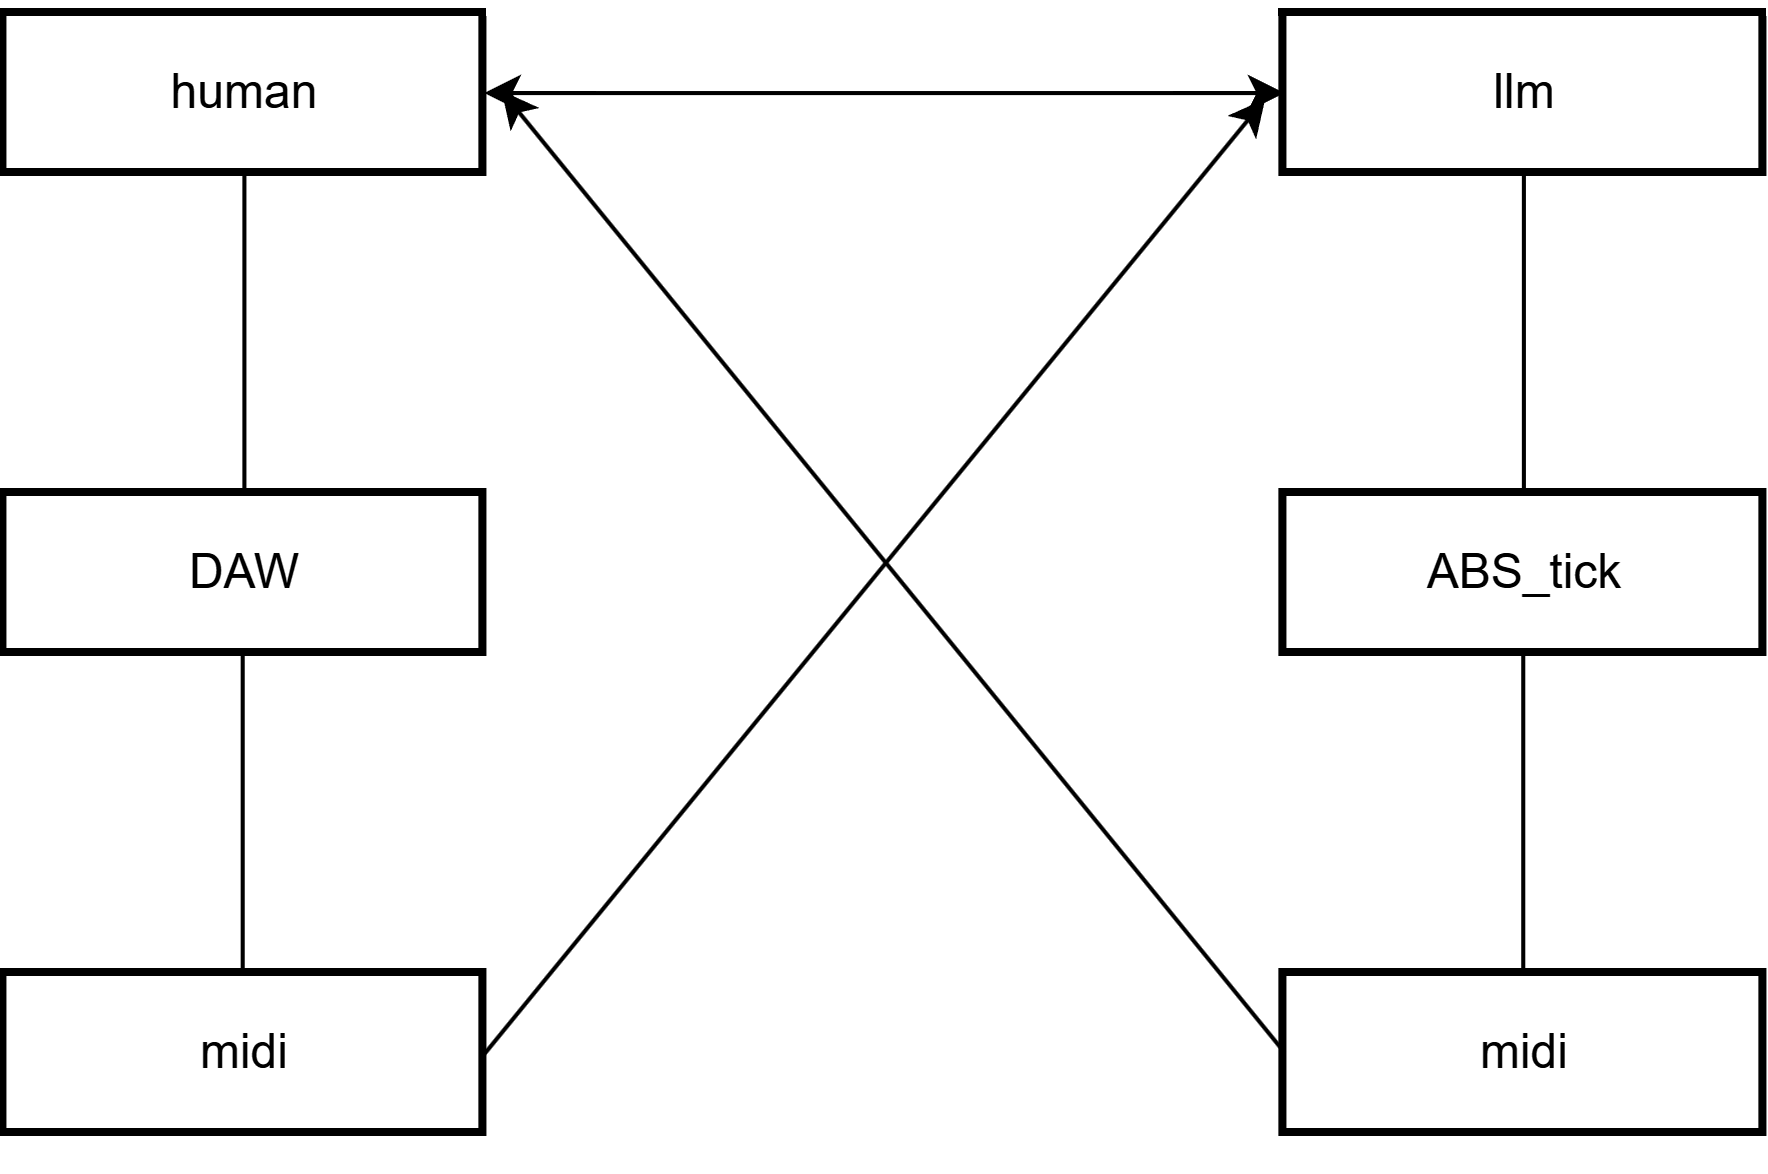
\includegraphics[width=0.54\textwidth]{fig4-hitl.png}
\caption{The coordinate round trip in the human--AI interaction path.}
\label{fig:hitl}
\end{figure}

\section{Discussion}
\label{sec:disc}

\subsection{The nature and the position of this work}

It is necessary to state the nature of this work truthfully. The mathematical essence of
the core coordinate system is the \textbf{piecewise evaluation of a piecewise linear
function}, which is trivial content; the only technical point is the relativisation of
the bar index within a segment $(M-A_s)$, and there is no non-trivial proof. It produces
no new mathematical knowledge; rather, it fixes a known but unformalised engineering
process into an invocable specification.

It is nevertheless still worth proposing separately, because that specification
\textbf{did not previously exist in explicit form}: DAW software implements it
internally but exposes only ``bar.beat''; writing that mapping as a closed form, giving
its degenerate property and explicitly drawing its applicability boundary is the work
done in this paper. The accurate statement is therefore: this coordinate system is not a
mathematical discovery but an $O(1)$ computational interface with clearly defined
boundaries, whose upper bound of value is determined by the time-signature change
density (section \ref{sec:domain}).

\subsection{Relation to existing representation systems}

The coordinate system of this paper does not replace the MIDI message stream or notation
description languages; it supplies the mapping layer between the two. MIDI takes
performance events as its unit of record, MusicXML takes the layout of the score as its
object of description, and neither provides an absolute position quantity independent of
the time signature; the absolute tick defined in this paper is exactly that missing
quantity.

\subsection{Potential impact on the formulation of music theory}

This paper does not claim that numbers should replace description, but it points out one
actual change: several concepts that could long be expressed only qualitatively acquire,
after coordinatization, a form that can be \textbf{counted pair by pair} --- the amount
of overlap, the pitch difference and the amount of gap (section \ref{sec:relation}). In
existing accounts these quantities rely on overall impressions such as ``a bit more
legato here'' or ``a bit more space here'', and overall impressions are hard to compare
and hard to reproduce. Once they have a quantitative form, they can at least be
compared, reproduced and modified locally.

\subsection{Limitations}

The scale of the experiments in this paper is limited, and the conclusions are
constrained by the following conditions.

\begin{enumerate}[leftmargin=2.2em,itemsep=0.15em,topsep=0.2em]
  \item Verification was completed on a single DAW only, and no cross-validation
        against other implementations has been carried out.
  \item No strict proof of the upper bound of the rounding error under a changing time
        signature has been given; only experimental observation is available
        (section \ref{sec:counter}).
  \item The correctness of the ``equidistance exclusion method'' in voice separation
        when three or more voices cross simultaneously has not been proved.
  \item The effectiveness of the semantic encapsulation layer in real teaching scenarios
        has not been verified by user studies.
  \item The collaborative case in section \ref{sec:case} is a single-case observation
        with no control group and no independent raters, and its conclusions should be
        treated as case evidence rather than a universal claim.
  \item The two worked examples of the generation architecture in section \ref{sec:gen}
        verify only the consistency of the formal constraints; no listening evaluation
        was carried out, and they constitute no claim about musicality.
\end{enumerate}

\subsection{Future work}

The following problems have a clear direction but were not resolved in this paper; they
are listed in order of priority.

\begin{enumerate}[leftmargin=2.2em,itemsep=0.15em,topsep=0.2em]
  \item Give an upper bound for the rounding error under a changing time signature, or
        prove that the error is identically zero for particular values of PPQ.
  \item Generalise the equidistance exclusion method to the case of several voices
        crossing simultaneously, or characterise its failure condition.
  \item Reproduce all the experiments on a second DAW, in order to test the
        implementation-independence of the conclusions.
  \item Design a listening experiment with a control group, in order to assess the
        actual musical effect of the proposed generation architecture.
\end{enumerate}

\section{Conclusion}
Starting from an observation of the DAW interface, this paper constructs the absolute
time coordinate system MATCS. The main conclusions are:

\begin{enumerate}[leftmargin=2.2em,itemsep=0.15em,topsep=0.2em]
  \item The position of a musical event can be translated into an absolute tick value
        independent of the time signature, the tempo and the tonality, whose form is
        given by equation \eqref{eq:abs};
  \item ``Irregular meter'' and ``variable time signature'' have different properties in
        tick mathematics, and the latter is the real cause of the failure of the original
        formula; under a changing time signature the original formula must be generalised
        to the piecewise summation form \eqref{eq:master}, of which the original formula
        is the degenerate special case at $n=1$;
  \item Taking ``the instant at which the vertical value changes'' as the sole criterion
        and redefining rests as empty events unifies the localization logic of notes and
        rests, and no undefined interval remains on the time axis;
  \item The applicability domain of that form is constrained by the time-signature
        change density: the parameter count grows linearly, and as the density approaches
        one change per bar the method must switch to a time-signature event table plus
        binary search;
  \item The reverse mapping cannot be replaced by hand calculation, and this is where
        the form is genuinely irreplaceable.
\end{enumerate}

Truthfully, the mathematical content of this paper is not substantial: its essence is
the piecewise evaluation of a piecewise linear function, the only technical point is the
relativisation of the bar index within a segment $(M-A_s)$, and there is no non-trivial
proof. Its contribution lies in fixing a known but unformalised engineering process into
a specification, and in clearly drawing its applicability boundary.



\appendix

\section{Excerpts from the research log}
This appendix excerpts, in chronological order, the original records made during the
derivation; several of the criteria in the main text arose from them.

\begin{quotedpassage}
\textbf{Day one · stability of the scale}. Observe the ``bar.beat.tick'' read-out in the
DAW over a long period: whether the time signature is modified, the tempo changed or the
material dragged, that read-out never changes and always points to the same absolute
position.
\end{quotedpassage}

\begin{quotedpassage}
\textbf{Day two · an attempt at formalisation}. The rudimentary form of equation
\eqref{eq:abs} was obtained, and the first beats of the second and third bars under
$4/4$ were substituted for checking, giving $3840$ and $7680$, in agreement with the
software read-out.
\end{quotedpassage}

\begin{quotedpassage}
\textbf{Day three · the counterexample}. After the time signature was changed from $4/4$
to $6/8$ the result showed a significant deviation, and dragging the material or moving
notes a long way failed in the same manner. Inspecting the deviation data revealed a
\textbf{determinate} error value between the two time signatures --- the error is
determinate rather than random, which shows that the model is not wrong but is missing a
variable.
\end{quotedpassage}

\begin{quotedpassage}
\textbf{Day three · the key observation}. An eighth note under $4/4$ has a span of
\texttt{0.0.50} in the read-out, while the same eighth note under $6/8$ reads
\texttt{0.1.00}. The two have the same tick length ($480$) but are interpreted as
different numbers of beats. The conclusion follows: the duration scale is not a global
constant but a local variable determined by the denominator of the time signature.
\end{quotedpassage}

\begin{quotedpassage}
\textbf{Day four · global localization}. Treat the DAW grid as a plane Cartesian
coordinate system: the horizontal axis is already given by the absolute tick, while the
vertical axis is still to be established. The difficulty of the vertical axis lies not
in labelling but in the criterion --- how to decide where a note begins and ends. This
yielded ``event $=$ the instant at which the vertical value changes''.
\end{quotedpassage}

\begin{quotedpassage}
\textbf{Day five · self-positioning}. Looking back at the form itself: its mathematical
essence is the piecewise evaluation of a piecewise linear function, which is trivial
content; the only technical point is the relativisation of the bar index within a
segment; and there is no non-trivial proof. Its value lies not in producing new
knowledge but in fixing a known process into an invocable specification.
\end{quotedpassage}

\section{Implementation of the core algorithm}
Construction of the piecewise axis and the bidirectional mapping (the original
implementation was in Lua; here it is transcribed into an equivalent form):

\begin{museCode}[language=Python]
def build_axis(sections, ppq):
    """sections: [(upToBar, bpi, denom), ...]; upToBar is strictly increasing"""
    axis, acc_bar, acc_tick = [], 0, 0
    for up_to, bpi, denom in sections:
        bars = up_to - acc_bar
        tpb = round(ppq * 4 / denom)
        axis.append(dict(from_bar=acc_bar + 1, to_bar=up_to, bars=bars,
                         bpi=bpi, tpb=tpb, start_tick=acc_tick,
                         ticks_per_bar=bpi * tpb))
        acc_bar = up_to
        acc_tick += bars * bpi * tpb
    return axis

def pos_to_tick(axis, bar, beat):
    for seg in axis:
        if bar <= seg["to_bar"]:
            rel = bar - seg["from_bar"]
            return seg["start_tick"] + (rel * seg["bpi"] + (beat - 1)) * seg["tpb"]
    raise ValueError("bar out of axis range")

def tick_to_pos(axis, tick):
    for i, seg in enumerate(axis):
        seg_end = seg["start_tick"] + seg["bars"] * seg["ticks_per_bar"]
        if tick < seg_end or i == len(axis) - 1:
            local = tick - seg["start_tick"]
            bar_off = local // seg["ticks_per_bar"]
            rem = local - bar_off * seg["ticks_per_bar"]
            beat = rem // seg["tpb"] + 1
            return seg["from_bar"] + bar_off, beat
    raise ValueError("tick out of axis range")
\end{museCode}

\section{Glossary of terms}
\begin{longtable}{@{}p{3.4cm}p{11.1cm}@{}}
\caption{Core terminology}\label{tab:glossary}\\
\toprule
\thd{Term} & \thd{Meaning} \\
\midrule
\endfirsthead
\multicolumn{2}{@{}l}{\small\itshape (continued)}\\
\toprule
\thd{Term} & \thd{Meaning} \\
\midrule
\endhead
\bottomrule
\endlastfoot
MATCS & Mozun Absolute Time Coordinate System, the absolute time coordinate system proposed in this paper \\
absolute tick & the tick count from the start of the project to that event, independent of the time signature, the tempo and the tonality \\
empty event & an event whose pitch attribute is empty and which has explicit onset and offset times; a rest is one example \\
event chain & the uninterrupted sequence formed by the end of each event meeting the start of the next \\
TPB & the number of numerical coordinate units per beat, $=\mathrm{PPQ}\times 4/\mathrm{Denom}$ \\
BPI & Beats Per Bar, the number of beats per bar, equal to the numerator of the time signature \\
PPQ & Pulses Per Quarter Note, the system's preset time resolution \\
Denom & the denominator of the time signature, which determines what kind of note ``one beat'' corresponds to \\
simple meter & $2/4$, $3/4$ etc., a single group of accents \\
compound meter & $6/8$, $9/8$, $12/8$, each ``beat'' being a dotted note \\
irregular meter & $5/8$, $7/8$, unequal division within the bar, the time signature itself unchanged \\
\textbf{variable time signature} & the signature is changed mid-piece and must be handled segment by segment \\
segment table & the prior metadata recording $n_k,p_k,d_k$ for each time-signature segment \\
segment start $S_s$ & the cumulative tick boundary at the start of segment $s$ \\
anchor & the reference position chosen when measuring relative distances \\
vertical value & the pitch state at a given absolute tick, $0$ denoting a rest \\
tick\_translate & the bidirectional mapping engine between the position representation and the absolute coordinate \\
line\_for\_llm & the structured semantic encapsulation layer for language models \\
\end{longtable}
\end{document}

\end{document}
